\chapter{Samples, setup and experiments}
\label{ch:experiments}

All the experiments have been carried out on \acs{PIC} developed within a FP7 project (IRIS, \cite{testa2016design}) that aimed to develop an optical router.
An optical router is a matrix of microresonators whose resonances are tuned at will to (re)direct an optical signal along a predefined path.
We exploit the nonlinear optical response of these nodes to demonstrate the feasibility of an all optical nonlinear activation function made on PIC.

%All the experiments have been carried out on samples manufactured for the IRIS project \cite{testa2016design}.
%This is due to the fact that in the time frame of this work there would have not been enough time to design and produce an ad hoc device.
%Moreover, as already stated, the aim of this thesis is to produce a proof of concept for an all-optical implementation of an activation function, rather than to construct a complete prototype.
%With the knowledge obtained during this work, future researches could design new structures by focusing on the correct parameters.

\section{The samples}
The IRIS project studied the design and the implementation of an integrated reconfigurable silicon photonics switch matrix, a routing device, as a replacement for electronic devices used in the telecommunication industry.
The completed integrated photonic circuit consists of a matrix of waveguides crossing each other and linked by couples of racetrack resonators, thermally-controlled.
At the ends of the waveguides other structures, interleavers and \acsp{AWG}, allowed many signals at different wavelengths to be multiplexed/demultiplexed onto/from the same waveguide.

\begin{figure}[hbtp]
	\centering
	\tikzsetexternalprefix{tikz/}	% set subfolder
\tikzsetnextfilename{IRIS}
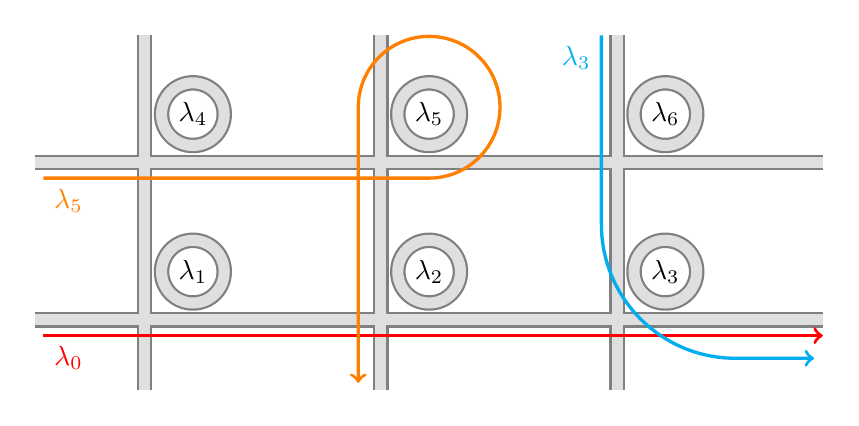
\begin{tikzpicture}[
		baseline,
		wave/.style	={ 
			very thick, line cap=butt, ->,
			%rounded corners=128pt,
		},
		guide/.style 	={ double=gray!25, double distance=4pt,
			thick, draw=black!50,
			rounded corners=4pt, line join=round, line cap=butt,
		},
		ring/.style 		={ circle, radius=64pt,
			double=gray!25, double distance=4pt,
			thick, draw=black!50,
			rounded corners=8pt, line join=round,
		},
	]
	
	\def\mylist{ 0/0/1, 3/0/2, 6/0/3, 0/2/4, 3/2/5, 6/2/6}
	
	% draw rings
	\foreach \x/\y/\n in \mylist
		\node [ring] (ring_\n) at (\x,\y) {$\lambda_\n$};
	
	% draw waveguides
	\draw [guide]
			% insert the horizontal wgs here
			(ring_1.south)++(-2,-0.2) -- ++(10,0)
			(ring_4.south)++(-2,-0.2) -- ++(10,0)
			% insert the vertical wgs here
			(ring_1.west)++(-0.2,-1.5) -- ++(0,4.5)
			(ring_2.west)++(-0.2,-1.5) -- ++(0,4.5)
			(ring_3.west)++(-0.2,-1.5) -- ++(0,4.5);
			
	% draw waves
	\draw [wave, red] (ring_1.south)++(-1.9,-0.4) node [below right] {$\lambda_0$} -- ++(9.9,0);
	\draw [wave, orange] (ring_4.south)++(-1.9,-0.4) node [below right] {$\lambda_5$} -- ++(4.9,0)
				arc (-90:180:0.9) -- ++(0,-3.5);
	\draw [wave, cyan] (ring_6.west)++(-0.4, 1) node [below left] {$\lambda_3$} -- ++(0,-2.4)
				arc (180:270:1.7) -- ++(1,0);
	
\end{tikzpicture}

	\caption{Scheme of a routing node of the full \acs{PIC} of IRIS. $\lambda_0$ travels from the input port to the through port; $\lambda_5$ is redirected from the input port to the drop port; $\lambda_3$ is redirected from an add port to the through port.}
	\label{fig:fullmatrix}
\end{figure}

Each node of the matrix can be modeled by a microring resonator in \acs{ADF} configuration (see \autoref{ssec:Microring_optical_cavity}).
Any signal that enters a node detuned from the resonance of the microring is directed toward the through port of the node.
On the other hand, any signal that enters a node in resonance with the microring is redirected toward the drop port.
\autoref{fig:fullmatrix} shows the scheme of a node in the full \acs{PIC}, where the signals is routed.

%The complexity of such photonic circuit required outstanding precision in the design and the fabrication.
%Hence, for preliminary testing purposes, each and every structure of which the full device is composed, has been manufactured repeatedly with several small variations.
%For example, several microrings in the \ac{ADF} configuration have been fabricated with different radius, or different ring-waveguide gap.
%The collection of all these testing structures on the same chip was produced in a few samples.
%All these test structures as well as a fully completed switch matrix were disposed on a single chip, accessible via grating couplers.

\newpage
The development of the final IRIS chip has required several steps of improvement and few generation of test samples were fabricated with different optical properties.
Thus the first step of the thesis has been to choose, among the many different devices available, the most promising ones.
%characterize qualitatively the response of some devices among the single structures, the short sequences of structures, and the full switch matrix itself.
%After many trials of different devices, my final choice was to study a system of intermediate complexity.
%In fact, since the work in this thesis is like the first step in a long journey, with this choice I tried to obtain a compromise between simplicity in immediate future (current work) and adaptability in the long term.
%For example, the current structure allowed me to study the nonlinear activation function, but could be reused in the future to study the weighted sum.
The structure selected (nicknamed \textit{mini-matrix}) is shown in \autoref{fig:photos} and it is composed by: a waveguide, coupled to eight drop channels through ring resonators.
In this family of devices, there were mini-matrices built with single microrings, double microrings, single racetracks, or double racetracks.
%The final choice was to study the \textit{mini-matrix} in which the coupling mechanism was provided by single ring resonators, because of its simpler transfer function in respect to double microrings or double racetracks.
\autoref{fig:minimatrix_scheme} shows a simplified scheme of the \textit{mini-matrix}.

\begin{figure}[htbp]
	\centering
	\begin{subfigure}[b]{0.7\textwidth}
		\centering
		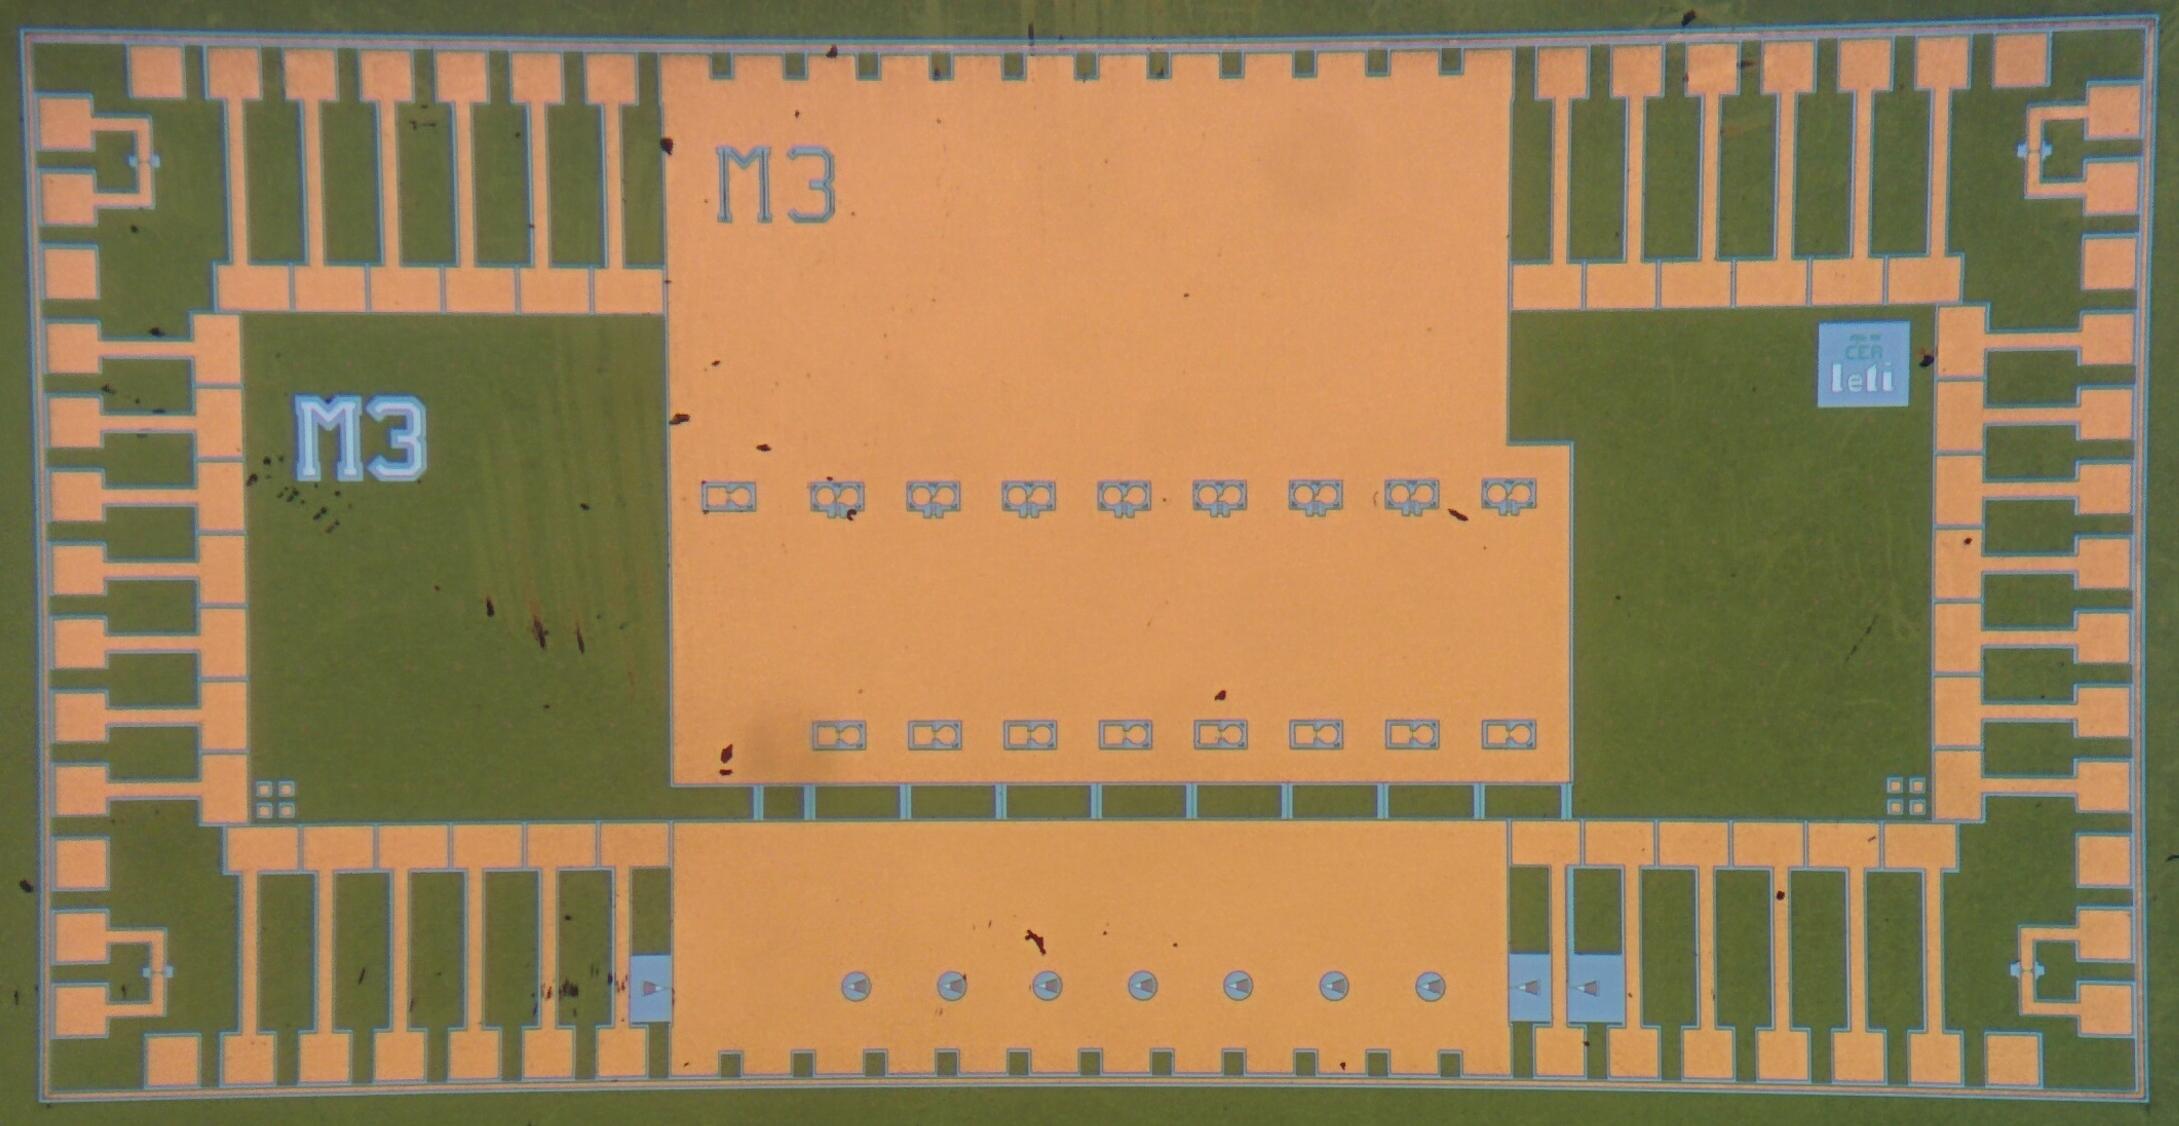
\includegraphics[width=\textwidth]{photos/minimatrix.png}
		\caption{mini-matrix}
		\label{fig:photo_minimatrix}
	\end{subfigure}
	\begin{subfigure}[t]{0.345\textwidth}
		\centering
		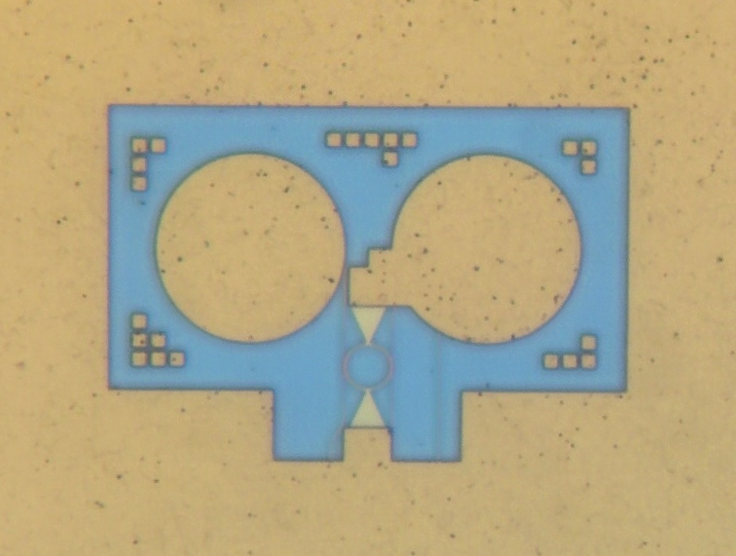
\includegraphics[width=\textwidth]{photos/ring.png}
		\caption{microring}
		\label{fig:photo_ring}
	\end{subfigure}
	\begin{subfigure}[t]{0.345\textwidth}
		\centering
		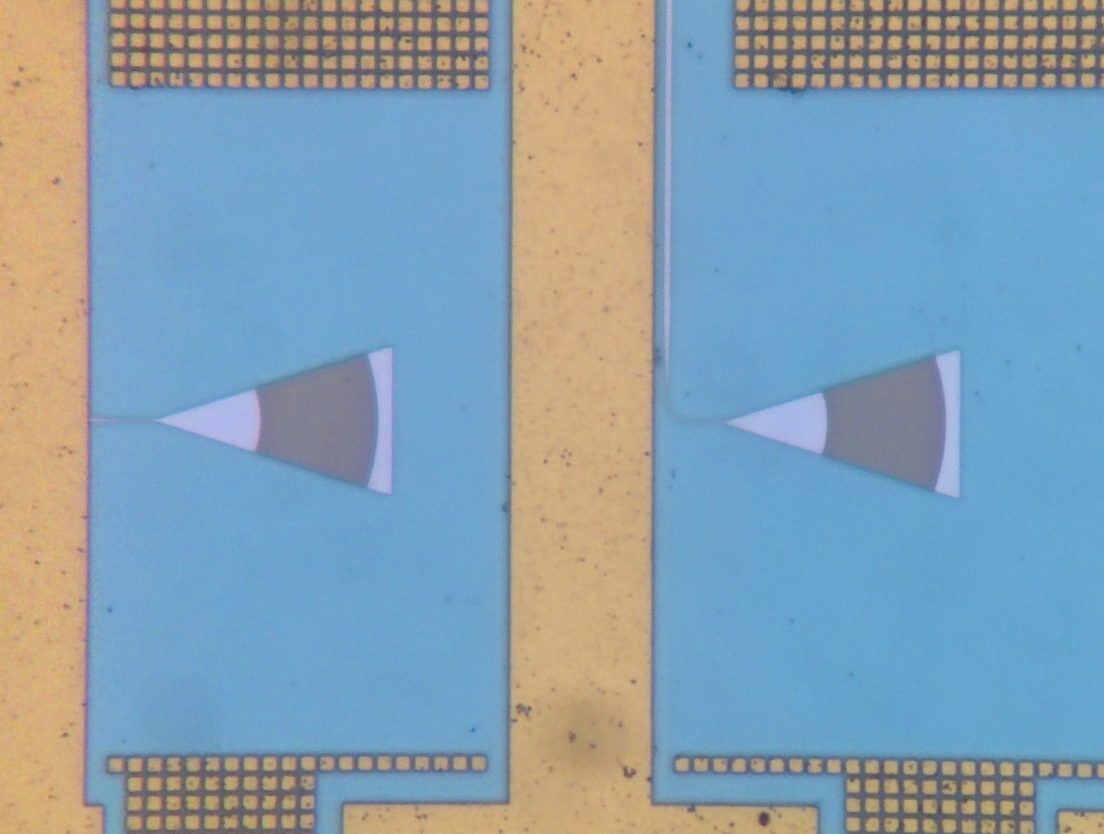
\includegraphics[width=\textwidth]{photos/grating.png}
		\caption{grating}
		\label{fig:photo_grating}
	\end{subfigure}
	\caption{Magnified photograph of the \textit{mini-matrix} device chosen (a) and two important structures: (b) microring resonator and (c) output grating couplers. }
	\label{fig:photos}
\end{figure}

\begin{figure}[hbtp]
	\centering
%	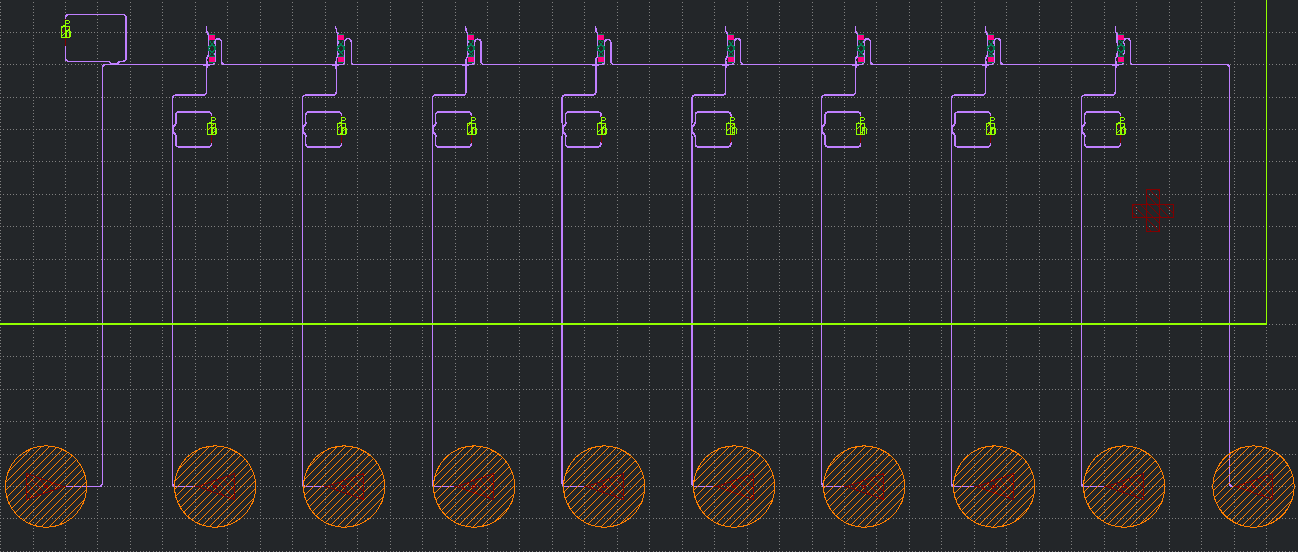
\includegraphics[scale=.4]{figures/miniMATRIX_Klayout.png}\\
	\tikzsetexternalprefix{tikz/}	% set subfolder
\tikzsetnextfilename{miniMATRIX_scheme}
\begin{tikzpicture}[
		baseline,
		grating/.style	={ isosceles triangle, rotate=180,
			draw=orange, preaction={fill, white},
			pattern color=orange, pattern=north west lines,
			thick,
			inner sep=0pt,	minimum size=12pt
		},
		guide/.style 	={ double=gray!25, double distance=1pt,
			thick, draw=black!50,
			rounded corners=4pt, line join=round, line cap=round,
		},
		ring/.style 		={ circle, radius=16pt,
			double=gray!25, double distance=1pt,
			thick, draw=black!50,
			rounded corners=8pt, line join=round,
		},
	]
	
	\def\mylist{	1/0.0/0, 2/1.5/0, 3/3.0/0, 4/4.5/0,
									5/6.0/0, 6/7.5/0, 7/9.0/0, 8/10.5/0}

	% declare node of gratings and coupling regions
	\node (input) at (-2,0) {};
	\foreach \name/\px/\py in \mylist {
			\draw (\px,\py) node (dr\name) {} ++(-0.2,2.5) node (cr\name) {};
		}
	\draw (12.0,0) node (th) {};

	% draw rings
	\foreach \name/\px/\py in \mylist {
			\node (r\name) [ring] at (cr\name) {};
			\node at (r\name.north) [above] {$r_\name$};
			\draw (cr\name.west) ++(-0.02,0) node (rL\name) {};
			\draw (cr\name.east) ++(+0.02,0) node (rR\name) {};
		}
		
	% draw waveguides
	\draw [guide] (input) to (-1.4,0) -- (-1.4,2)
			% insert all the bendings here
			-| (rR1.east) -- ++(0,.4) -- ++(.3,0) -- ++(0,-0.9)
			-| (rR2.east) -- ++(0,.4) -- ++(.3,0) -- ++(0,-0.9)
			-| (rR3.east) -- ++(0,.4) -- ++(.3,0) -- ++(0,-0.9)
			-| (rR4.east) -- ++(0,.4) -- ++(.3,0) -- ++(0,-0.9)
			-| (rR5.east) -- ++(0,.4) -- ++(.3,0) -- ++(0,-0.9)
			-| (rR6.east) -- ++(0,.4) -- ++(.3,0) -- ++(0,-0.9)
			-| (rR7.east) -- ++(0,.4) -- ++(.3,0) -- ++(0,-0.9)
			-| (rR8.east) -- ++(0,.4) -- ++(.3,0) -- ++(0,-0.9)
			-- (11.4,2) -- (11.4,0) -- (th);

	\foreach \name/\px/\py in \mylist {
			\draw [guide] (dr\name) -| (rL\name.west) -- ++(0,0.4)  -- ++(120:0.2);
		}
	\foreach \px in {-.51,.99,2.49,3.99,5.49,6.99,8.49,9.99}
		\node [shape=diamond, draw=gray!25, fill=gray!25, inner sep=.8pt] at (\px,2) {};
	
	% draw gratings
	\node (grin) at (input) [grating, rotate=180] {};
	\node at (grin.south) [below left] {$in$};
	\foreach \name/\px/\py in \mylist{
			\node (gr\name) [grating] at (dr\name) {};
			\node at (gr\name.north) [below right] {$dr_\name$};
		}
	\node (grth) at (th) [grating] {};
	\node at (grth.north) [below right] {$th$};

	% draw highlighted areas
	\draw [thick, draw=purple, fill=purple!50, opacity=0.4] (r1)
				++(-0.4,-0.3) rectangle ++(0.8,0.6);
	\draw [thick, draw=blue, fill=blue!50, opacity=0.4]
				(.84,1.85) rectangle ++(0.3,0.3);
	
\end{tikzpicture}
	\caption{
		Simplified scheme of the \textit{mini-matrix} integrated photonic circuit (structures are not in scale).
		Triangles (orange) are the grating couplers ($in$, $dr_{1-8}$, $th$).
		Waveguides and rings ($r_{1-8}$) are shown as thick grey lines.
		The bigger (purple) highlighted area is a coupling region, shown in \autoref{fig:minimatrix_scheme_zoom}.
	}
	\label{fig:minimatrix_scheme}
\end{figure}

The resonance of each microring is strictly defined by the design of the structure, however it is ultimately changed by imperfections and uncertainties of the manufacturing process.
Hence, since the optical router requires precise positioning of the resonances, their fine tuning is obtained by controlling the temperature of the material.
Each one of the microring resonators in the structure has been manufactured with a thermo-electric heater, which is used to produce the thermo-optic effect (see \autoref{ssec:Thermal_nonlinearities}) in order to induce the required resonance tuning \cite{testa2016design}.
\autoref{fig:minimatrix_scheme_zoom} shows the scheme of the microring resonator geometry, without any non-optical structures (e.g. heaters, metallic contacts).
%This feature has never been exploited in this work, but could come of use in the future.

\begin{figure}[htbp]
	\centering
%	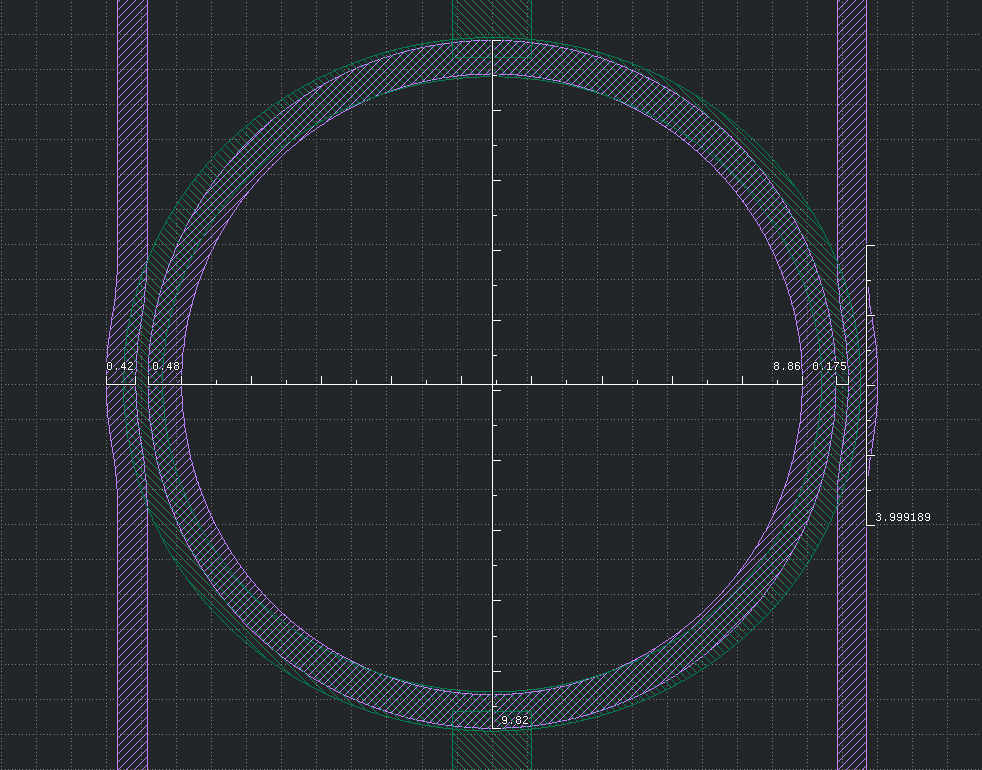
\includegraphics[scale=.4]{figures/single_ring_zoom.png}\\
	\tikzsetexternalprefix{tikz/}	% set subfolder
\tikzsetnextfilename{miniMATRIX_scheme_zoom}
\begin{tikzpicture}[
		baseline,
		scale=0.6,
		every pin edge/.style={-},
	]

%	\draw [help lines] (-3,-3) grid (3,3);
	
	\filldraw [draw=black!50, fill=gray!20, even odd rule]
		(0,0) circle [radius=4.43, thick]
		(0,0) circle [radius=4.91, thick];
	\path [name path=inner] (0,0) circle [radius=5.085];
	\path [name path=outer] (0,0) circle [radius=5.505];
	%distance between waveguides is 9.848
	\path [name path=leftwg]  (-4.924,-6) rectangle (-5.344,+6);
	\path [name path=rightwg] (+4.924,-6) rectangle (+5.344,+6);
	
	\path [name intersections={of=inner and leftwg, name=leftyin}];
	\path [name intersections={of=outer and leftwg, name=leftyout}];
	
	\path [name intersections={of=inner and rightwg, name=rightyin}];
	\path [name intersections={of=outer and rightwg, name=rightyout}];
	
	\draw [black!50, line join=round, rounded corners=1pt, fill=gray!20]
		(-4.924,-6) -- (-5.344,-6) -- (leftyout-4)
		.. controls ++(+103:1) and ++(-103:1) .. (leftyout-2)
		-- (-5.344,+6) -- (-4.924,+6) -- (leftyin-1)
		.. controls ++(-102:1) and ++(+102:1) .. (leftyin-2)
		-- cycle;
	
	\draw [black!50, line join=round, rounded corners=1pt, fill=gray!20]
		(+4.924,-6) -- (+5.344,-6) -- (rightyout-4)
		.. controls ++(+77:1) and ++(-77:1) .. (rightyout-2)
		-- (+5.344,+6) -- (+4.924,+6) -- (rightyin-1)
		.. controls ++(-78:1) and ++(+78:1) .. (rightyin-2)
		-- cycle;
	
	\draw [-stealth] (0,0) -- ++(60:4.43) node [left, midway] {$R_{in}$};
				
	\draw [|-|,black, thick] (+4.430,+0) -- (+4.910,+0) node [pin=+60:\SI{0.48}{\um}] {};
	\draw [|-|,black, thick] (+4.924,-3) -- (+5.344,-3) node [pin=+60:\SI{0.42}{\um}] {};
	\draw [|-|,black, thick] (-4.924,+0) -- (-5.085,+0) node [pin=120:\SI{0.175}{\um}] {};
	
	\draw [thick, -stealth] (+6.0,-6) -- (+6.0,-5) node [midway, right] {in};
	\draw [thick, -stealth] (+6.0,+5) -- (+6.0,+6) node [midway, right] {through};
	\draw [thick, -stealth] (-6.0,-5) -- (-6.0,-6) node [midway, left] {drop};
	\draw [thick, -stealth] (-6.0,+6) -- (-6.0,+5) node [midway, left] {add};

\end{tikzpicture}
	\caption{
	Microring optical cavity region, structures are in scale.
	The ring has an internal radius of $R_{in}=\SI{4.43}{\um}$ and its width is of \SI{0.48}{\um}.
	The waveguides side coupled to the ring have a width of \SI{0.42}{\um} and distance from the ring of \SI{.175}{\um}.
	}
	\label{fig:minimatrix_scheme_zoom}
\end{figure}

\subsection{Initial characterization}
\label{ssec:initial_characterization}
To obtain an initial characterization of the sample, I arranged an experimental setup to measure its fundamental attributes, such as the \acf{FSR}, the \acf{FWHM}, and the $Q$ factor of the resonances.
These features can all be obtained through a study of the transmitted intensity in the through and drop channels, shown in \autoref{fig:minimatrix_scheme}.
A scheme of the experimental setup used is showed in \autoref{fig:simple_setup}.

\begin{figure}
	\centering
	\tikzsetnextfilename{simple_setup}

% Define size/space
\def\loopsize{.8cm}
\def\loopoffset{0.2cm}
% Define the loops
\def\myloops#1#2{
\begin{scope}[shift={#1}, scale=#2]
        % Draw the baseline
    \draw (-\loopoffset,0) -- (\loopoffset,0);
        % Draw the loops
    \draw (-\loopoffset,0)	node [draw, thick, circle, anchor=south, minimum size=\loopsize] (id) {};
    \draw (0,0) 						node [draw, thick, circle, anchor=south, minimum size=\loopsize] (id) {};
    \draw (\loopoffset,0) 	node [draw, thick, circle, anchor=south, minimum size=\loopsize] (id) {};
\end{scope}
}

\begin{tikzpicture}
	[
	source/.style ={
		draw, rectangle, inner sep=6pt, anchor=west
		},
	VOA/.style ={
		draw, circle, inner sep=2pt, fill=white, anchor=west
		},
	sample/.style={
		draw, chamfered rectangle, chamfered rectangle=8pt, anchor=west
		},
	coupler/.style={
		draw, rounded rectangle, rounded rectangle right arc=none, anchor=west, inner sep=2pt
		},
	thick,
	] %radius=5, inner sep=0pt,	minimum size=3mm}
	
	\draw (0,0) node [source, align=center] (tunics) {\small TUNICS}
					node [above] at (tunics.north) {source}
				(tunics.east)
%				++(0.6, 0) node [source] (eydfa) {EYDFA}
%					node [above] at (eydfa.north) {amplifier}
%				(eydfa.east)
				++(0.6, 0) node [VOA] (circ) {$\scriptstyle\circlearrowright$}
%					node [above] at (circ.north) {circ}
			  (circ.east)
				++(1.2, 0) node (polarizer) {}
				++(1.2, 0) node [coupler] (couplerA) {\tiny(a)}
					node [above] at (couplerA.north east) {\tiny .5}
					node [below] at (couplerA.south east) {\tiny .5}
			   +(1.0,-1.2) node [source] (osa) {OSA}
					node [right] at (osa.east) {detector}
				(couplerA.east)
				++(0.6, 0) node [sample] (sample) {sample}
				(sample.east)
				++(0.6, 0) node [source] (detectorA) {PD-A}
					node [above] at (detectorA.north) {detector};
	
	\myloops{(polarizer)}{1}
	\node [below] at (polarizer) {polarizer};

	\draw (tunics) -- ++(circ)
				(circ) node [above left] {\tiny (1)}
				(circ) node [above right] {\tiny (2)}
				(circ) to [out=225, in=90] ++(-0.4,-0.6) node [circle, inner sep=1pt, black, fill=black] {}
																								node [below] {\tiny (3)}
				(circ) to [out=315, in=90] ++(+0.4,-0.6) node [circle, inner sep=1pt, black, fill=black] {}
																								node [below] {\tiny (4)}
				(circ) -- (polarizer)
				(polarizer) to (couplerA)
				(couplerA.20) to [out=0, in=180] (sample)
				(couplerA.-20) to [out=0, in=180] (osa)
				(sample) -- (detectorA)
				;

\end{tikzpicture}
	\caption{Scheme of the setup used to obtain an initial characterization of the optical nodes.
		%The source is an external cavity tunable laser that produces a laser beam of up to \SI{8}{\mW} in the range of wavelength required (\SIrange{1500}{1580}{\nm}).
		The source is an external cavity tunable laser that produces a laser beam in the range \SIrange{1500}{1580}{\nm}.
		The second element is an optical circulator and the third is a fiber polarizer.
		After the signal is split into two arms (50\%:50\%): one goes to an \acs{OSA} and is used as reference during the measurements, while the other is fed into the sample.
		Finally the intensity of the signal passed through the node is read by a Germanium \acs{PD} (PD-A).
		}
	\label{fig:simple_setup}
\end{figure}

The laser source used in this measures is an external cavity Yamatsu TUNICS T-100S tunable infrared laser.
It produces a linearly polarized continuous wave laser beam of optical power up to \SI{8}{\mW} in the wavelength range \SIrange{1500}{1580}{\nm}, with a minimum wavelength step of \SI{1}{\pm}.
The generated light is injected into an optical circulator to protect the laser cavity from back-reflections.
A circulator is a device that works similarly to a roundabout: input signals from the first port are directed only toward the second port. Similarly, signals injected in the second port are guided in the third port only and so on.
The circulator used in the setup has four ports.
Afterwards the beam is divided into two equal parts by means of a fiber coupler: one is analyzed by an Anritsu 9710C \ref{} \acf{OSA} and the other is brought to the sample.
The output of the sample is coupled in a fiber and taken to the (PD-A) infrared \ac{PD}

The presence of an \ac{OSA} after the source is due to the fact that the self-referencing mechanism of the laser that occurs during its initialization was not reliable.
In fact, I observed that measures of the resonance taken in different days (after reinitializing the source) showed different values for the resonance.
Hence I analyzed the wavelength emitted from the source with the OSA and observed that
the actual wavelength emitted deviated rather sensibly from the supposed one.
In order to correct this problem, I sampled the supposed-actual wavelength relationship with the \ac{OSA}, and then I implemented an online correction by exploiting the its inverse function.
In doing so, I assumed the \ac{OSA} as a reference.
\autoref{fig:tunics} shows a typical calibration, where the emitted wavelength is greater than the actual one at shorter wavelengths but smaller at longer ones.

\begin{figure}[thbp]
	\centering
	\tikzsetexternalprefix{tikz/}	% set subfolder
\tikzsetnextfilename{TUNICS}

\begin{tikzpicture}[	baseline,
										spy using outlines={circle, magnification=5, connect spies}
										]
	
	\begin{axis}[
			title={Source Calibration},
			xlabel={Source Wavelength [\si{\nm}]},
			ylabel={OSA Wavelength [\si{\nm}]},
%			tick align=outside,
%			tick pos=left,
			width=\textwidth*0.75,%
			height=207pt,
			legend pos = outer north east,
			cycle list name=color list,
			/pgf/number format/1000 sep=,
			grid = major,
			ytick={1510, 1520, 1530, 1540, 1550, 1560, 1570},
		]
    
%		\addlegendentry{\hspace{-.6cm}output}
%		\addlegendimage{empty legend};
	  
		\addplot [black, domain=1510:1570, forget plot] {x};
    \addplot [red, mark=*] table [x index=0, y index=1] {tikz/tunics_calibration.csv};
    \addlegendentry{ $y=mx+q$ }
		\addlegendentry{\hspace{-.6cm}m=0.9425}
		\addlegendimage{empty legend};
		\addlegendentry{\hspace{-.6cm}q=87.4754}
		\addlegendimage{empty legend};
		\addlegendentry{\hspace{-.6cm}standard error}
		\addlegendimage{empty legend};
		\addlegendentry{\hspace{-.6cm}0.0005}
		\addlegendimage{empty legend};

		% slope=0.9425054945054935,
		% intercept=87.47538461538625,
		% rvalue=0.999998547069192,
		% pvalue=8.306111526948216e-32,
		% stderr=0.0004844238149507297

		% 1533 resonance
		\draw [orange] (1532.675, {1532.675-0.2375}) -- (1532.675, {1532.675+0.2375});
		
		\coordinate (spypoint33) at (1532.675,1532.675);
%		\coordinate (magnifyglass33) at (1525,1555);
		\coordinate (magnifyglass33) at (1545,1525);

		% 1552 resonance
		\draw [orange] (1551.900, {1551.900-0.3}) -- (1551.900, {1551.900+0.3});
		
		\coordinate (spypoint52) at (1551.9,1551.9);
%		\coordinate (magnifyglass52) at (1555,1525);
		\coordinate (magnifyglass52) at (1565,1525);
    
	\end{axis}
	
	\spy [cyan, size=2cm] on (spypoint33) in node[fill=white] at (magnifyglass33);	
	\spy [cyan, size=2cm] on (spypoint52) in node[fill=white] at (magnifyglass52);	
	
\end{tikzpicture}
	\caption{Typical wavelength dependence calibration.
	The black line shows the identity.
	The orange segments in the magnified frames represent the \acs{FWHM} of the resonances.}
	\label{fig:tunics}
\end{figure}

All the structures built on the test chip are accessible via grating couplers and are designed to support modes in the \acs{TE} polarization only.
Grating couplers are planar periodic structures engineered to couple proper light bandwidth from free space into integrated waveguides and vice versa.
In my case, the grating transmission is maximum for wavelengths from \SIrange{1540}{1550}{\nm} and decreases outside.
%This means that even though the PIC could work in a broader range of wavelength, we are limited by the transmission efficiency of each grating.
The coupling loss per grating is almost \SI{5}{\dB} at the maximum transmission, i.e. a third of the signal power is lost at each coupling.

\newpage
\begin{figure}[htbp]
	\centering
	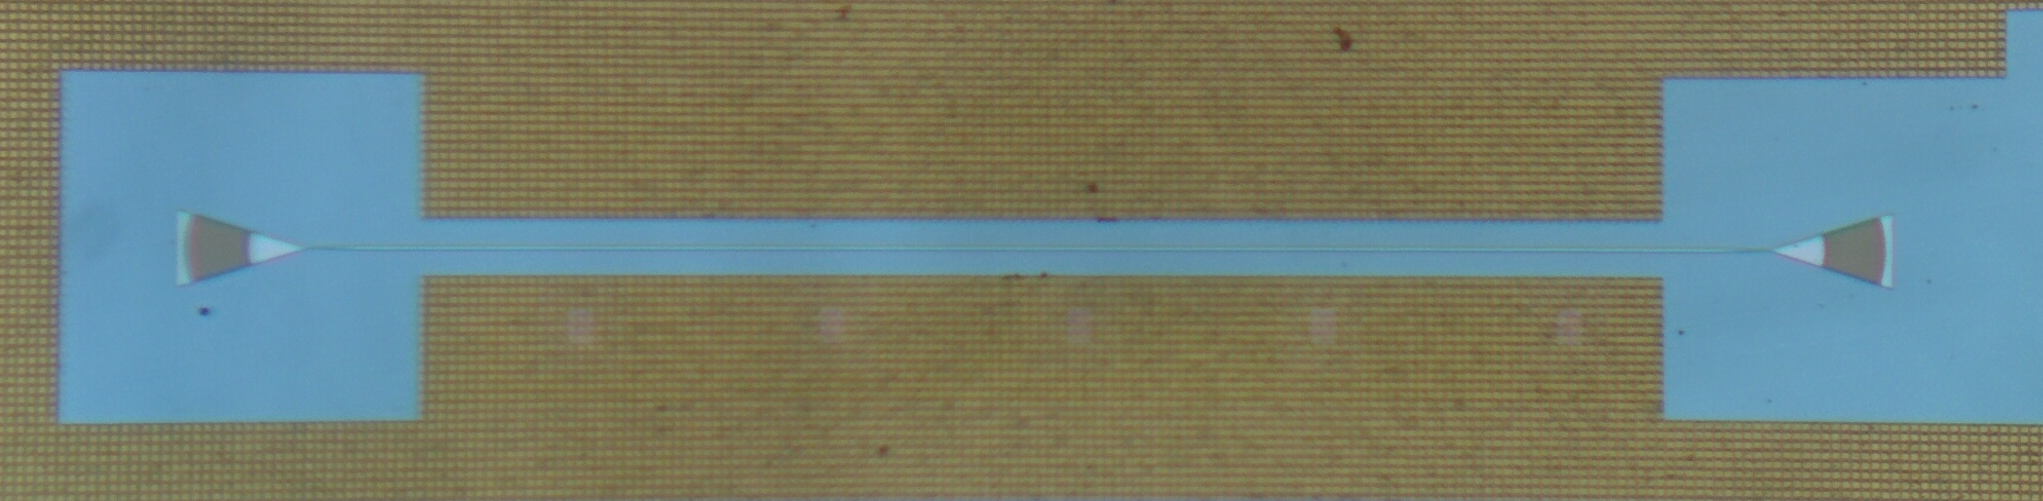
\includegraphics[width=0.7\textwidth]{photos/gg.png}
	\caption{Grating transmission efficiency test structure.}
	\label{fig:grating-grating}
\end{figure}

To properly characterize the coupler transmission, I used a structure manufactured for this purpose.
Depicted in \autoref{fig:grating-grating}, it consists of an input grating coupler, a straight waveguide, and an output grating coupler.
Its transmission efficiency is shown in \autoref{fig:grating}.

%This means that light at wavelength in the predefined range, impinging on the grating coupler with the correct angle, is coupled inside the waveguide on the \ac{PIC}.
%Similarly, light coming from a waveguide to a grating coupler, is radiated as plane wave from the grating coupler with the same mentioned angle.

\begin{figure}[hbtp]
	\centering
	\tikzsetexternalprefix{tikz/}	% set subfolder
\tikzsetnextfilename{grating}

\begin{tikzpicture}[	baseline]
	
	\begin{axis}[
			title={Grating Transmission Efficiency},
			xlabel={Wavelength [\si{\nm}]},
			ylabel={Transmission Efficiency},
%			tick align=outside,
%			tick pos=left,
			width=\textwidth*0.75,%
			height=207pt,
			legend pos = outer north east,
			cycle list name=color list,
			/pgf/number format/1000 sep=,
			yticklabels={,,0.06,0.08,0.1,0.12},
		]
    
%		\addlegendentry{\hspace{-.6cm}output}
%		\addlegendimage{empty legend};
	  
%		\addplot [black, domain=1510:1570, forget plot] {x};
    \addplot [red, mark=*] table [x index=0, y index=1] {tikz/grating.csv};
%    \addlegendentry{ $y=mx+q$ }
    
	\end{axis}
	
\end{tikzpicture}
	\caption{The maximum transmission efficiency is around \num{0.117} and the coupling loss per grating is almost \SI{5}{\dB}, average over five consecutive measures.}
	\label{fig:grating}
\end{figure}

The sample is adjusted on a 2-\acs{DOF} linear stage in between two 3-\acs{DOF} linear stages that holds the input and output coupling fibers.
\autoref{fig:alignment} shows the respective positions of the input and the output fibers in respect to the grating couplers.

\begin{figure}[!hbtp]
	\centering
	\tikzsetnextfilename{alignment}

\def\sx{6}
\def\sy{2}
\def\cx{0.4}
\def\cy{0.2}

\begin{tikzpicture}[	baseline,
%										x={(0.866cm,-0.5cm)},	y={(0.866cm,0.5cm)},	z={(0cm,1cm)},
										x={(0.9cm,-0.05cm)},		y={(0.3cm,+0.5cm)},	z={(0cm,1cm)},
										line join=round,
										]
\tikzstyle{paddle}=[very thick, fill=white,line join=round]
\coordinate (O) at (0, 0, 0);

% fiber in
%\draw[thick] (0,-1.5,0) to[out=30,in=220] (1,0,0);

% sample
\draw[white, preaction={fill, white}, pattern=crosshatch dots, pattern color=gray!50]
	++(0,-\sy,0) -- ++(\sx,0,0) -- ++(0,\sy,0) -- ++(0,\sy,0) -- ++(-\sx,0,0) -- cycle;
\draw[-stealth] (0.2,-1.8,0) -- ++(0.5,0.0,0) node [below] {$\scriptstyle x$};
\draw[-stealth] (0.2,-1.8,0) -- ++(0.0,0.5,0) node [left]  {$\scriptstyle y$};

\draw[black, double=white, double distance=1.2pt, rounded corners=6pt]
			(1.8,0,0) -- ++(0.7,0,0) -- ++(0,-1,0) --
			++(1,0,0) -- ++(0,1,0) -- ++(0.7,0,0);

% grating couplers
\node (coupler1) at (2,0,0) {};
\node (coupler2) at (4,0,0) {};
\draw[orange, preaction={fill, white}, pattern=north east lines, pattern color=orange]
			++(2,0,0) -- ++(-\cx,-\cy,0) -- ++(0,\cy,0) -- ++(0,\cy,0) -- cycle;
\draw[orange, preaction={fill, white}, pattern=north east lines, pattern color=orange]
			++(4,0,0) -- ++(+\cx,-\cy,0) -- ++(0,\cy,0) -- ++(0,\cy,0) -- cycle;

\draw[white, fill=white]
	++(2.9,-1.8,0) -- ++(0.2,0,0) -- ++(0,3.6,0) -- ++(-0.2,0,0) -- cycle;

\draw 	(1.8,0,0) -- ++(0,0,1.4)
			(4.2,0,0) -- ++(0,0,1.4);
\draw 	[dashed]
			(1.8,0,1.4) -- ++(0,0,.7)
			(4.2,0,1.4) -- ++(0,0,.7);

%0.970295726 * 1.3 = 1.261384444, 0.241921896 * 1.3 = 0.314498464
\draw 	(1.8,0,0) -- ++(-0.34,0,1.36)
			(4.2,0,0) -- ++(+0.34,0,1.36);
\draw 	[dashed]
		 	(1.8,0,0) ++(-0.34,0,1.36) -- ++(-.17,0,.68) node (in) {}
			(4.2,0,0) ++(+0.34,0,1.36) -- ++(+.17,0,.68) node (out) {};

\draw[red,very thick] ++(1.8,0,0) +(0,0,1)
	\foreach \t in {91,92,...,104}
		{-- +(+{cos(\t)},0,{sin(\t)})};

\draw[red,very thick] ++(4.2,0,0) +(0,0,1)
	\foreach \t in {91,92,...,104}
		{-- +(-{cos(\t)},0,{sin(\t)})};

% red light
\fill[red!15,draw=red,very thick,opacity=0.5] ++(0.25,0,0)
	node [circle,inner sep=1pt,red,fill=red, opacity=0.5] {}
	+(0,0.55,0) % core
	\foreach \t in {90,95,100,...,450}
		{--+({0.54*cos(\t)},{0.55*sin(\t)},0)}--cycle
	(0,0,1)
	++({0.3*cos(30)*cos(14)},{0.3*sin(30)},{0.3*cos(30)*sin(14)})
	-- ({0.25+0.54*cos(30)},{0.55*sin(30)},0)
	(0,0,1)
	++({0.3*cos(210)*cos(14)},{0.3*sin(210)},{0.3*cos(210)*sin(14)})
	-- ({0.25+0.54*cos(180+30)},{0.55*sin(180+30)},0);
%	;

% left fiber
% lower surface
\fill[blue!15,draw=blue,very thick,opacity=0.5] ++(0,0,1)
		+(0,1,0) % cladding
		\foreach \t in {90,95,100,...,450}
			{--+({cos(\t)*cos(14)},{sin(\t)},{cos(\t)*sin(14)})}--cycle;
\fill[blue!15,draw=blue,very thick,opacity=0.75] ++(0,0,1)
		+(0,0.3,0) % core
		\foreach \t in {90,95,100,...,450}
			{--+({0.3*cos(\t)*cos(14)},{0.3*sin(\t)},{0.3*cos(\t)*sin(14)})}--cycle;
% inner surface
\draw[draw=blue,very thick, opacity=0.75] ++(0,0,1)
	++({0.3*cos(30)*cos(14)},{0.3*sin(30)},{0.3*cos(30)*sin(14)})
	-- ++(-.17,0,.68)
	(0,0,1)
	++({0.3*cos(210)*cos(14)},{0.3*sin(210)},{0.3*cos(210)*sin(14)})
	-- ++(-.17,0,.68);
% external surface
\draw[draw=blue,very thick, opacity=0.5] ++(0,0,1)
	++({cos(30)*cos(14)},{sin(30)},{cos(30)*sin(14)})
	-- ++(-.23,0,.91)
	(0,0,1)
	++({cos(210)*cos(14)},{sin(210)},{cos(210)*sin(14)})
	-- ++(-.23,0,.91);

% right fiber
% lower surface		
\fill[blue!15,draw=blue,very thick,opacity=0.5] ++(6,0,1)
	+(0,1,0) % cladding
	\foreach \t in {90,95,100,...,450}
		{--+({cos(\t)*cos(-14)},{sin(\t)},{cos(\t)*sin(-14)})}--cycle;
\fill[blue!15,draw=blue,very thick,opacity=0.75] ++(6,0,1)
	+(0,0.3,0) % core
	\foreach \t in {90,95,100,...,450}
		{--+({0.3*cos(\t)*cos(-14)},{0.3*sin(\t)},{0.3*cos(\t)*sin(-14)})}--cycle;
% inner surface
\draw[draw=blue,very thick, opacity=0.75] ++(6,0,1)
	++({0.3*cos(+5)*cos(-14)},{0.3*sin(+5)},{0.3*cos(+5)*sin(-14)})
	-- ++(+.17,0,.68)
	(6,0,1)
	++({0.3*cos(180+5)*cos(-14)},{0.3*sin(180+5)},{0.3*cos(180+5)*sin(-14)})
	-- ++(+.17,0,.68);
% external surface
\draw[draw=blue,very thick, opacity=0.5] ++(6,0,1)
	++({cos(+5)*cos(-14)},{sin(+5)},{cos(+5)*sin(-14)})
	-- ++(+.23,0,.91)
	(6,0,1)
	++({cos(180+5)*cos(-14)},{sin(180+5)},{cos(180+5)*sin(-14)})
	-- ++(+.23,0,.91);

\draw[-stealth] (-1,-2.5,1) -- ++(0.5,0.0,0.0) node [below] {$\scriptstyle x$};
\draw[-stealth] (-1,-2.5,1) -- ++(0.0,0.5,0.0) node [right]  {$\scriptstyle y$};
\draw[-stealth] (-1,-2.5,1) -- ++(0.0,0.0,0.5) node [left]  {$\scriptstyle z$};
	
\draw[-stealth] (+7,-2.5,1) -- ++(0.5,0.0,0.0) node [below] {$\scriptstyle x$};
\draw[-stealth] (+7,-2.5,1) -- ++(0.0,0.5,0.0) node [right]  {$\scriptstyle y$};
\draw[-stealth] (+7,-2.5,1) -- ++(0.0,0.0,0.5) node [left]  {$\scriptstyle z$};
	
\end{tikzpicture}

	\caption{Alignment phase of the input and output fibers over the corresponding grating couplers.
	The optical fibers are aligned at an angle of \ang{14} over the grating couplers in such a way to inject and collect as much light as possible.
	The sample was placed in a specific slot of a copper sample holder, which was secured onto a 2-\acs{DOF} manual stage.
	The two fiber holders were placed on a 3-\acs{DOF} manual stage each, to align them properly.
	}
	\label{fig:alignment}
\end{figure}

\newpage
Once secured the input and output optical fibers in place on the linear stages, the alignment phase begins.
First the source light is positioned at a wavelength that transmit on the correct channel, for example the resonance wavelength transmit in the drop channels but not in the through channel and vice versa.
Then the optical fibers are carefully moved in the respective positions that maximize the coupled signal.
The alignment have to be checked periodically, many times a day, to compensate for mechanical relaxations of the setup.
%This procedure needs meticulous practice and method to avoid errors due to noise and imprecise movements of the linear stages.
%Moreover, sometimes the procedure must be repeated even if neither the sample nor the fibers have been moved, because of mechanical relaxation processes of the inner gears.

To obtain the best results, I also designed a new modular fiber holder with fixed angle (\autoref{fig:holders}) that was manufactured twice, one for each fiber. %, that could be used more easily than the older ones with adjustable angle.
The main body has been manufactured in aluminum, except for the actual part that sustains the fiber, which was produced in iron.
The metallic tip of the holder, appropriately grooved to house the optical fiber, can hold still the fiber with the help of little magnets.
This technique aims at reducing as much as possible the vibrations of the fibers ends, which causes fluctuations in the amount of light coupled to the gratings.

\begin{figure}[htbp]
	\centering
	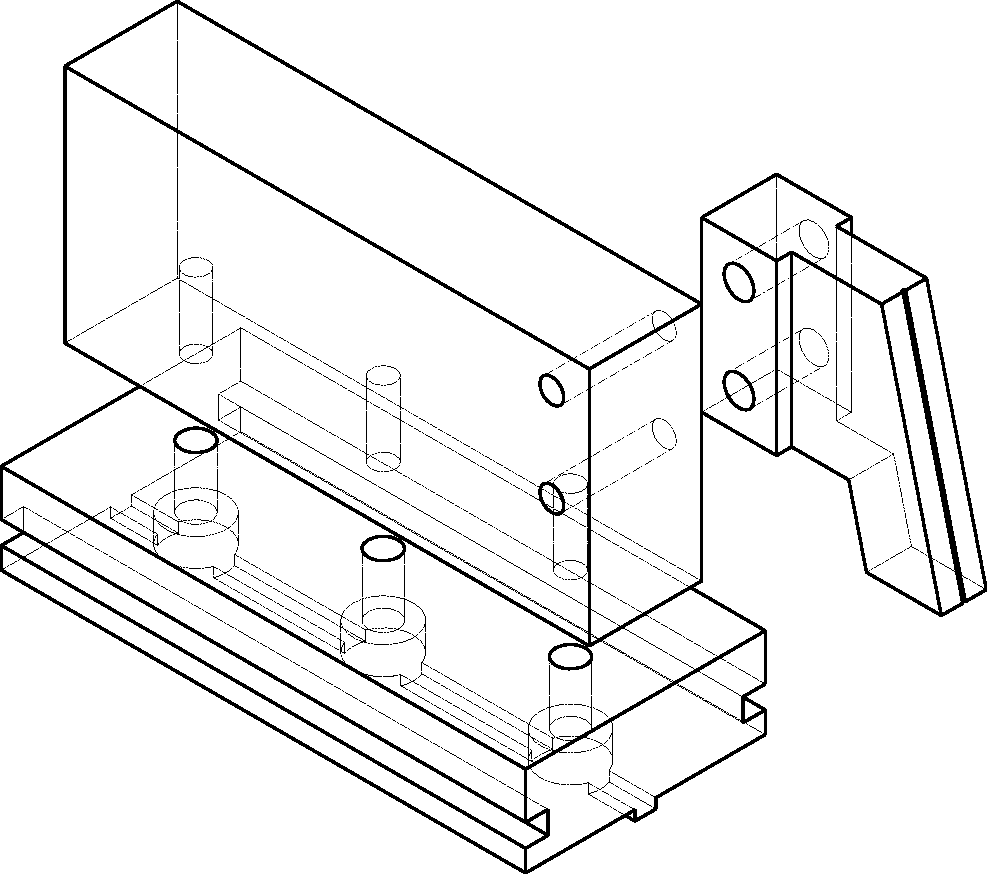
\includegraphics[height=8cm]{figures/supporto_completo.pdf}
	\caption{Exploded-view drawing of the fiber holder design.
	The holder is composed by three pieces.
	The tip is made of iron, in order to be used together with small magnets.}
	\label{fig:holders}
\end{figure}

Since the \acp{PIC} developed for IRIS support \acs{TE} modes only, after the positions of the optical fibers have been optimized, the coupled signal is maximized by the use of a polarizer.
The polarizer, placed between the fiber coupler and the sample, is a device composed by a long optical fiber.
Such fiber is coiled in three separate loops which have the effect of a half-wave plate, one quarter-wave plate, and another half-wave plate respectively.
Each coil can be manipulated, in a similar manner to the bulky quater-/half-wave plates, to change the output (linear) polarization of the light.
%The position of the polarization stage before of after the \ac{OSA} junction is not relevant as the \ac{OSA} is polarization independent.

In order to further reduce the impact of noise on measures, I also boxed the three linear stages with a rigid enclosure.
This decreased the noise, due to the movement of the fiber tips in air by at least one order of magnitude.

For the initial characterization, I studied the response of each output at input signals with low optical power and in the working range of the grating couplers, to identify the position of the resonances and their shape.
%As shown in \autoref{fig:M3sweep}, the through channel $th$ follows the shape of the grating coupler response, which is centered around \SI{1540}{\um} and slowly drops with the growing relative distance from that wavelength.
\autoref{fig:M3sweep} shows the normalized transmission of the eight drop channel ($dr_1$ to $dr_8$ ) and the through channel ($th$).
The first drop channel ($dr_1$) has the expected lorentzian shape, with a free spectral range of $FSR=\SI{19.2+-.1}{\nm}$, while the shapes of all the other drop channels are highly distorted because of the light collected by $dr_1$.
%On the other hand, all the other drop channels show a transmission that is perturbed by the light collected in the first channel.

\begin{figure}[htbp]
	\centering
%	\tikzsetexternalprefix{tikz/}	% set subfolder
\tikzsetnextfilename{M1}

\begin{tikzpicture}[baseline]

	\definecolor{color1}{rgb}{0.12156862745098,0.466666666666667,0.705882352941177}
	\definecolor{color2}{rgb}{1,0.498039215686275,0.0549019607843137}
	\definecolor{color3}{rgb}{0.172549019607843,0.627450980392157,0.172549019607843}
	\definecolor{color4}{rgb}{0.83921568627451,0.152941176470588,0.156862745098039}
	\definecolor{color5}{rgb}{0.580392156862745,0.403921568627451,0.741176470588235}
	\definecolor{color6}{rgb}{0.549019607843137,0.337254901960784,0.294117647058824}
	\definecolor{color7}{rgb}{0.890196078431372,0.466666666666667,0.76078431372549}
	\definecolor{color8}{rgb}{0.45,0.45,0.45}
	\definecolor{color9}{rgb}{0.25,0.25,0.99}
	
	\begin{axis}[
			title={Output Power},
			xlabel={Wavelength [\si{\nm}]},
			ylabel={Output Power [\si{\uW}]},
			tick align=outside,
			tick pos=left,
			width=\textwidth*0.75,%
			height=207pt,
			legend pos = outer north east,
			cycle list name=color list,
		]
    
		\addlegendentry{\hspace{-.6cm}output}
		\addlegendimage{empty legend};
		\addlegendentry{\hspace{-.6cm}channel}
		\addlegendimage{empty legend};
		
%	  \pgfplotstableread[col sep=tab]{tikz/M1.csv}\tableM1
	  
    \pgfplotsinvokeforeach{1,2,...,8}{
        \addplot [semithick, color#1] table [x index=0, y index=#1] {tikz/M1.csv};
        \addlegendentryexpanded{ $dr_#1$ }
    }
		\addplot [semithick, color9] table [x index=0,y index=9] {tikz/M1.csv};
    \addlegendentry{ $th$ }
    
	\end{axis}
\end{tikzpicture}
%	\tikzsetexternalprefix{tikz/}	% set subfolder
\tikzsetnextfilename{M2}

\begin{tikzpicture}[baseline]

	\definecolor{color1}{rgb}{0.12156862745098,0.466666666666667,0.705882352941177}
	\definecolor{color2}{rgb}{1,0.498039215686275,0.0549019607843137}
	\definecolor{color3}{rgb}{0.172549019607843,0.627450980392157,0.172549019607843}
	\definecolor{color4}{rgb}{0.83921568627451,0.152941176470588,0.156862745098039}
	\definecolor{color5}{rgb}{0.580392156862745,0.403921568627451,0.741176470588235}
	\definecolor{color6}{rgb}{0.549019607843137,0.337254901960784,0.294117647058824}
	\definecolor{color7}{rgb}{0.890196078431372,0.466666666666667,0.76078431372549}
	\definecolor{color8}{rgb}{0.45,0.45,0.45}
	\definecolor{color9}{rgb}{0.25,0.25,0.99}
	
	\begin{axis}[
			title={Output Power},
			xlabel={Wavelength [\si{\nm}]},
			ylabel={Output Power [\si{\uW}]},
			tick align=outside,
			tick pos=left,
			width=\textwidth*0.75,%
			height=207pt,
			legend pos = outer north east,
			cycle list name=color list,
		]
    
		\addlegendentry{\hspace{-.6cm}output}
		\addlegendimage{empty legend};
		\addlegendentry{\hspace{-.6cm}channel}
		\addlegendimage{empty legend};
		
%	  \pgfplotstableread[col sep=tab]{tikz/M1.csv}\tableM1
	  
    \pgfplotsinvokeforeach{1,2,...,8}{
        \addplot [semithick, color#1] table [x index=0, y index=#1] {tikz/M2.csv};
        \addlegendentryexpanded{ $dr_#1$ }
    }
		\addplot [semithick, color9] table [x index=0,y index=9] {tikz/M2.csv};
    \addlegendentry{ $th$ }
    
	\end{axis}
\end{tikzpicture}
	\tikzsetexternalprefix{tikz/}	% set subfolder
\tikzsetnextfilename{M3}

\begin{tikzpicture}[baseline]

	\definecolor{color1}{rgb}{0.12156862745098,0.466666666666667,0.705882352941177}
	\definecolor{color2}{rgb}{1,0.498039215686275,0.0549019607843137}
	\definecolor{color3}{rgb}{0.172549019607843,0.627450980392157,0.172549019607843}
	\definecolor{color4}{rgb}{0.83921568627451,0.152941176470588,0.156862745098039}
	\definecolor{color5}{rgb}{0.580392156862745,0.403921568627451,0.741176470588235}
	\definecolor{color6}{rgb}{0.549019607843137,0.337254901960784,0.294117647058824}
	\definecolor{color7}{rgb}{0.890196078431372,0.466666666666667,0.76078431372549}
	\definecolor{color8}{rgb}{0.45,0.45,0.45}
	\definecolor{color9}{rgb}{0.25,0.25,0.99}
	
	\begin{axis}[
			title={Output Power},
			xlabel={Wavelength [\si{\nm}]},
			ylabel={Transmission},
%			tick align=outside,
%			tick pos=left,
			width=\textwidth*0.75,%
			height=207pt,
			legend pos = outer north east,
			cycle list name=color list,
			/pgf/number format/1000 sep=,
			xtick distance=3,
			minor x tick num=2,
			minor y tick num=1,
		]
    
		\addlegendentry{\hspace{-.6cm}output}
		\addlegendimage{empty legend};
		\addlegendentry{\hspace{-.6cm}channel}
		\addlegendimage{empty legend};
		
%	  \pgfplotstableread[col sep=tab]{tikz/M1.csv}\tableM1
	  
    \pgfplotsinvokeforeach{1,2,...,8}{
        \addplot [semithick, color#1] table [x index=0, y index=#1] {tikz/m3.csv};
        \addlegendentryexpanded{ $dr_#1$ }
    }
		\addplot [semithick, color9] table [x index=0,y index=9] {tikz/m3.csv};
    \addlegendentry{ $th$ }
    
	\end{axis}
\end{tikzpicture}
	\caption{
		Transmission spectra of the drop channels ($dr_1$ to $dr_8$) and through channel $th$, average over five consecutive measures.
		The $dr_1$ channel shows the expected shape, whereas the other drop channels are clearly disturbed by the first one.
		The through channel shows a shape similar to the expected one, but it is actually the results of all the drop channels.
	}
	\label{fig:M3sweep}
\end{figure}

Another interesting fact is that the peak transmission of $dr_1$ channel is higher than the maximum transmission of $th$.
This is due to two factors: primarily the coupling maximization process with the linear stages has a repeatability error of about \SI{10}{\percent}, secondarily the $th$ channel is a longer structure and hence its losses are expected to be higher than the 'shorter` $dr_1$ channel.

Since $dr_1$ is the only channel with an unperturbed transmission, I focused my attention on its response only.
Specifically, I studied the resonance near \SI{1551.9}{\um}: % because it was the one with the highest transmitted signal and hence provided a better \acs{SNR}.
\autoref{fig:M3_1550_resonance} shows such resonance and highlights its center $\lambda_{res}=\SI{1551.9+-0.1}{\nm}$ and width $FWHM=\SI{0.6+-0.05}{\nm}$.
The estimated quality factor is $Q=\num{2600+-200}$.

\begin{figure}[!hbtp]
	\centering
	\tikzsetexternalprefix{tikz/}	% set subfolder
\tikzsetnextfilename{M3resonance}

\begin{tikzpicture}[baseline]

	\definecolor{color1}{rgb}{0.12156862745098,0.466666666666667,0.705882352941177}
%	\definecolor{color2}{rgb}{1,0.498039215686275,0.0549019607843137}
%	\definecolor{color3}{rgb}{0.172549019607843,0.627450980392157,0.172549019607843}
%	\definecolor{color4}{rgb}{0.83921568627451,0.152941176470588,0.156862745098039}
%	\definecolor{color5}{rgb}{0.580392156862745,0.403921568627451,0.741176470588235}
%	\definecolor{color6}{rgb}{0.549019607843137,0.337254901960784,0.294117647058824}
%	\definecolor{color7}{rgb}{0.890196078431372,0.466666666666667,0.76078431372549}
%	\definecolor{color8}{rgb}{0.45,0.45,0.45}
%	\definecolor{color9}{rgb}{0.25,0.25,0.99}
	
	\begin{axis}[
			title={Transmission},
			xlabel={Wavelength [\si{\nm}]},
			ylabel={Transmission},
			width=\textwidth*0.75,%
			height=207pt,
			legend pos = outer north east,
			xmin=1548, xmax=1556,
			/pgf/number format/1000 sep=,
		]
    
		\addlegendentry{\hspace{-.6cm}output}
		\addlegendimage{empty legend};
		\addlegendentry{\hspace{-.6cm}channel}
		\addlegendimage{empty legend};
		
%	  \pgfplotstableread[col sep=tab]{tikz/M1.csv}\tableM1
	  
		\addplot [semithick, cyan] table [x index=0, y index=1] {tikz/res1552.csv};
		\addlegendentryexpanded{ $dr_1$ }
		
		\draw [<-] ({1551.9+0.30+0.1}, 0.306) -- ({1551.9+1.5}, 0.306)
				node [right] {\small $FWHM$}; 
		\draw [<-] ({1551.9-0.4-0.1}, 0.306) -- ({1551.9-1.5}, 0.306);
    
	\end{axis}
\end{tikzpicture}
	\caption{
		Resonance at \SI{1551.9}{\nm}, transmission to the drop port $dr_1$, average over five consecutive measures.
%		This spectrum is the only one unperturbed by the other transmission spectra.
%		The FWHM and the resonance wavelength are clearly visible in the figure.
	}
	\label{fig:M3_1550_resonance}
\end{figure}

\section{Characterization of the Activation Function}
\label{sec:Characterization_of_the_Activation_Function}
To characterize the nonlinear response of the microring resonator the setup used for the initial measures has been modified.
To induce the thermal bistability effect in the microring the signal of the TUNICS has been amplified using an \ac{EYDFA}.
%Even more so with the addition of the optical amplifier, the role of the circulator placed between the sources and the rest of the devices is of fundamental importance.
In this configuration, the role of the circulator placed between the sources and the rest of the devices acquires even more importance, as back-reflected signals that enter optical amplifier in the wrong direction can cause serious damage to the equipment.

In addition to the amplifying stage, a remotely controlled \ac{VOA} was added between the polarizer and the sample, to quantitatively characterize the nonlinear response of the microring. %the response of the microring resonator to signals of fixed wavelength but different optical power.
The \ac{VOA} employed is controlled by a voltage signal in the range \SIrange{0}{5}{\V}: it provides full transparency for \SI{0}{\V} and full attenuation for \SI{5}{\V} and, in between, the attenuator behaves similarly to a sigmoid function, shown in \autoref{fig:VOA}.
This curve has been identified with its closest analytical polynomial, to obtain an inverse formula that links transparency values in the range $[0,1]$ to the respective correct voltage value.

\begin{figure}[htbp]
	\centering
	\tikzsetexternalprefix{tikz/}	% set subfolder
\tikzsetnextfilename{VOA}

\begin{tikzpicture}[	baseline ]
	
	\begin{axis}[
			title={VOA Calibration},
			xlabel={Control Signal [\si{\V}]},
			ylabel={VOA Transparency},
			width=\textwidth*0.75,%
			height=207pt,
			legend pos = outer north east,
		]
		
    \addplot [mark=+] table [x index=0, y expr=\thisrowno{1}/1.519545] {tikz/VOA_calibration.csv};
    
	\end{axis}
	
\end{tikzpicture}
	\caption{Typical calibration curve of the attenuation curve of the VOA.
		The data has been fitted with a spline to implement online control over the attenuation value.
	}
	\label{fig:VOA}
\end{figure}%1.519545

This setup successfully induces the nonlinear response in the microring for detunings up to values comparable to half $FWHM$.
However, instabilities of the source and the amplification stages in the optical power and in the wavelength of the signal increase the uncertainty on the measures.
Specifically, the system shows a drift in optical power immediately after the source and amplification stages are switched on and random noise (e.g. \SI{5}{\uW} of noise over \SI{1}{\mW} at the detector).
Moreover, the wavelength of the light generated shows a slow drift toward shorter wavelengths, which becomes important for long measurements.
The typical wavelength stability of the source is rated at \SI[per-mode=symbol]{+-3}{\pico\meter\per\hour} (from instrument datasheet).

The first corrective measure is obtained by allowing the system to thermalize.
The most critical instrument is the \ac{EYDFA}, which might take up to half an hour to reach a steady state.
This step reduces the slow drift in the output power of the source, but does not suppress the instantaneous noise in power and wavelength of the signal.

In order to provide a correction for the instantaneous noise, a small part of the signal is collected from the main path, before the VOA, via a fiber coupler (99\%:1\%) and it is the equally distributed via a second fiber coupler (50\%:50\%) to the OSA and to a second infrared \ac{PD} (PD-B).
The completed setup is shown in \autoref{fig:pump_setup}.

\begin{figure}[hbtp]
	\centering
	\tikzsetnextfilename{pump_setup}

% Define size/space
\def\loopsize{.8cm}
\def\loopoffset{0.2cm}
% Define the loops
\def\myloops#1#2{
\begin{scope}[shift={#1}, scale=#2]
        % Draw the baseline
    \draw (-\loopoffset,0) -- (\loopoffset,0);
        % Draw the loops
    \draw (-\loopoffset,0)	node [draw, thick, circle, anchor=south, minimum size=\loopsize] (id) {};
    \draw (0,0) 						node [draw, thick, circle, anchor=south, minimum size=\loopsize] (id) {};
    \draw (\loopoffset,0) 	node [draw, thick, circle, anchor=south, minimum size=\loopsize] (id) {};
\end{scope}
}

\begin{tikzpicture}
	[
	source/.style ={
		draw, rectangle, inner sep=6pt, anchor=west
		},
	VOA/.style ={
		draw, circle, inner sep=2pt, fill=white, anchor=west
		},
	sample/.style={
		draw, chamfered rectangle, chamfered rectangle=8pt, anchor=west
		},
	coupler/.style={
		draw, rounded rectangle, rounded rectangle right arc=none, anchor=west, inner sep=2pt
		},
	thick,
	] %radius=5, inner sep=0pt,	minimum size=3mm}
	
	\draw (0,0) node [source, align=center] (tunics)
									{\small TUNICS\\\tiny + \\\small EYDFA}
					node [above] at (tunics.north) {source}
					node [below] at (tunics.south) {amplified}
				(tunics.east)
%				++(0.6, 0) node [source] (eydfa) {EYDFA}
%					node [above] at (eydfa.north) {amplifier}
%				(eydfa.east)
				++(0.6, 0) node [VOA] (circ) {$\scriptstyle\circlearrowright$}
%					node [above] at (circ.north) {circ}
			  (circ.east)
				++(0.6, 0) node [coupler] (couplerA) {\tiny(a)}
					node [above] at (couplerA.north east) {\tiny .5}
					node [below] at (couplerA.south east) {\tiny .5}
			   +(1.0,-1.2) node [source] (osa) {OSA}
					node [below] at (osa.south) {detector}
				(couplerA.east)
				++(1.2, 0) node (polarizer) {}
				++(1.2, 0) node [coupler] (couplerB) {\tiny(b)}
					node [above] at (couplerB.north east) {\tiny .9}
					node [below] at (couplerB.south east) {\tiny .1}
				(couplerB.east)
				++(1.0, 0) node [VOA] (voa) {$\scriptstyle\nearrow$}
					node [above] at (voa.north) {voa}
			   +(0.0,-1.2) node [source] (detectorB) {Ge B}
					node [below] at (detectorB.south) {detector}
			  (voa.east)
				++(0.6, 0) node [sample] (sample) {sample}
				(sample.east)
				++(0.6, 0) node [source] (detectorA) {Ge A}
					node [above] at (detectorA.north) {detector};
	
	\myloops{(polarizer)}{1}
	\node [below] at (polarizer) {polarizer};

	\draw (tunics) -- ++(circ) node [pos=.85, above] {\tiny (1)}
				(circ) -- (couplerA) node [pos=.15, above] {\tiny (2)}
				(circ) to [out=225, in=90] ++(-0.4,-0.6) node [circle, inner sep=1pt, black, fill=black] {}
																								node [below] {\tiny (3)}
				(circ) to [out=315, in=90] ++(+0.4,-0.6) node [circle, inner sep=1pt, black, fill=black] {}
																								node [below] {\tiny (4)}
				(couplerA.20) to [out=0, in=180] (polarizer)
				(couplerA.-20) to [out=0, in=180] (osa)
				(polarizer) to (couplerB)
				(couplerB.20) to [out=0, in=180] (voa)
				(couplerB.-20) to [out=0, in=180] (detectorB)
				(voa) -- (sample)
				(sample) -- (detectorA)
				;

\end{tikzpicture}
	\caption{Scheme of the setup used to obtain characterization of the thermal bistability in the microring resonator.
		The source (TUNICS) is amplified by an \acs{EYDFA} and is followed by the circulator and by the polarizer.
		Then a small part of the signal is collected by a fiber coupler (99\%:1\%) and it is equally distributed between the OSA and an additional infrared \ac{PD} (PD-B).
		The signal in the main path passes through a \acf{VOA}, then it is injected into the sample, and finally extracted to be read by the first \ac{PD} (PD-A).
		}
	\label{fig:pump_setup}
\end{figure}

In this configuration, PD-B measures the instantaneous power in input at the VOA and, together with the value of transparency selected on the VOA, provides control over effective power coupled into the \ac{PIC} and correction over the noise in the power of the source.
The sampling rate of PD-B is the same of PD-A and is limited by the acquisition board (\SI{1}{\kHz}).

On the other hand, the \ac{OSA} provides a check over the wavelength of the source, but no correction can be implemented.
Moreover, the measures obtained by means of the \ac{OSA}, due to intrinsic limitations of the instrument and to the high complexity of the measure itself, have a much lower sampling rate in comparison to the measures given by the \acp{PD}.

Since this setup has been employed to measure several times the hysteresis cycle, for the same input wavelength, the measurement could run for several minutes consecutively.
In order to collect a significant number of points, without important drifts in the signal wavelength, the sampling time had to be reduced as much as possible.
For this reason, the \ac{OSA} has been employed as a check on the signal wavelength, before and after each measure of the hysteresis loops.

%On the other hand, the second infrared detector was inserted in the measuring loops such that it collected data for each sampled point.
To summarize, the data collected is composed by the optical power measured before the \ac{VOA}, by the transparency of the \ac{VOA}, and by the optical power measured at the output.
This three-point measurement allows more robustness against power fluctuations.

%Other than the addition discussed so far, the system setup is very similar to the one used before.
%The coupling system and alignment process of the sample are the same described above in \autoref{ssec:initial_characterization}.

\subsection{Bistability wavelength dependence}
\label{ssec:bistability_wavelength_dependence}
The first feature studied is the dependence of the overall shape of the bistability hysteresis loop on wavelength detuning.
As seen in \autoref{ssec:Simulations}, the form of the bistability changes with the detuning from the resonant wavelength.
This behavior is also observed in the transmission spectra experimentally measured, as shown in \autoref{fig:bistability_shape}.

\begin{figure}[hbtp]
	\centering
	\tikzsetexternalprefix{tikz/}	% set subfolder
\tikzsetnextfilename{shapes}

\newcommand{\plotshape}[1]{
    \pgfplotstableread[col sep=tab, header=true]{#1}{\table}
    \pgfplotstablegetcolsof{#1}
    \pgfmathtruncatemacro\numberofcols{\pgfplotsretval - 1}
    \pgfplotsinvokeforeach{1,...,\numberofcols}{
        \pgfplotstablegetcolumnnamebyindex{##1}\of{\table}\to{\colname}
        \addplot [semithick, color##1, mark=*, mark size=1]%
        		table [x index= 0, y index=##1] {#1};
        \addlegendentryexpanded{ \colname }
    }
}

\begin{tikzpicture}[baseline]

	\definecolor{color1}{rgb}{0.12156862745098,0.466666666666667,0.705882352941177}
	\definecolor{color2}{rgb}{1,0.498039215686275,0.0549019607843137}
	\definecolor{color3}{rgb}{0.172549019607843,0.627450980392157,0.172549019607843}
	\definecolor{color4}{rgb}{0.83921568627451,0.152941176470588,0.156862745098039}
	\definecolor{color5}{rgb}{0.580392156862745,0.403921568627451,0.741176470588235}
	\definecolor{color6}{rgb}{0.549019607843137,0.337254901960784,0.294117647058824}
	\definecolor{color7}{rgb}{0.890196078431372,0.466666666666667,0.76078431372549}
	\definecolor{color8}{rgb}{0.45,0.45,0.45}
	\definecolor{color9}{rgb}{0.25,0.25,0.99}
	\definecolor{color10}{rgb}{0.0,0.0,0.0}
	\definecolor{color11}{rgb}{0.12156862745098,0.466666666666667,0.705882352941177}
	\definecolor{color12}{rgb}{1,0.498039215686275,0.0549019607843137}
	\definecolor{color13}{rgb}{0.172549019607843,0.627450980392157,0.172549019607843}
	\definecolor{color14}{rgb}{0.83921568627451,0.152941176470588,0.156862745098039}
	\definecolor{color15}{rgb}{0.580392156862745,0.403921568627451,0.741176470588235}
	\definecolor{color16}{rgb}{0.549019607843137,0.337254901960784,0.294117647058824}
	\definecolor{color17}{rgb}{0.890196078431372,0.466666666666667,0.76078431372549}
	\definecolor{color18}{rgb}{0.45,0.45,0.45}
	\definecolor{color19}{rgb}{0.25,0.25,0.99}
	
	\begin{axis}[
			title={Internal Power},
			xlabel={Pump Power [\si{mW}]},
			ylabel={Internal Power [arb.units]},
%			tick align=outside,
			tick pos=left,
			width=\textwidth*0.75,%
			height=207pt,
			legend pos = outer north east,
			cycle list name=color list,
			forget plot style={opacity=0.4},
		]
		\addlegendentry{\hspace{-.6cm}$\Delta\lambda$ in \si{\pm}}
		\addlegendimage{empty legend};
		
		\plotshape{tikz/shapes.csv}
		
	\end{axis}
\end{tikzpicture}
	\caption{Many bistability loops at different wavelengths.
		The loops that are closer to the microring resonance have smaller bistability regions or they have not one at all.
		Loops that are farther from the resonance have larger bistability regions.}
	\label{fig:bistability_shape}
\end{figure}

As expected, the region of bistability disappears into a sigmoid for small detunings, while becomes larger for increased detunings.
The range of wavelengths with which the sample has been probed is upper limited due to the growing pump power required to activate the bistability.

Even though the behavior observed experimentally is similar to the one obtained with the simulations, there are some differences:
first of all, in the experiments the transmission for high input power saturates at the same value for different detunings.
Moreover, in the experiment all wavelengths shows a peak and a decrease in transmission from a certain level of input power.
On the contrary, in the simulations the output power does not saturate and shows different transmission efficiency for each detuning (see \autoref{fig:sim_bist_cycle}).

Several are the factors that might produce these discrepancies between the experiments and the simulations.
First of all, the setup and especially the sample are composed by many different structures.
Each of them has its unique response to high values of optical power.
Secondly, the parameters employed in the simulation are an estimate of the actual parameters that define the microring resonator and its coupling with the waveguides.
Lastly, the theoretical model implemented in the numerical calculations is an approximation of the physical phenomena that occur in the system.

\subsubsection{Bistability region edges}
\label{sssec:bistability_region_edges}
In order to precisely characterize the abrupt jumps on the edges of the bistability region, the stability of the system is crucial.
Hence I implemented a specific series of measurements, which samples only the nearest part of the edge: the amount of points sampled is smaller, however the complete measurement is faster and the sampling near the bistability edges is more dense.

The first step of each measurement is setting the source wavelength at a specific value, which is measured by the \ac{OSA}.
Then the serial measurements begins: for ascending loops, at the beginning \ac{VOA} is initialized at full attenuation and then is used to sample the edge with small increasing steps.
For descending loops, the \ac{VOA} is initialized at full transparency and the steps are decreasing instead.
After the predefined number of loops is completed, the wavelength of the source is measured with the \ac{OSA} again.
%These loops repeatedly initialized the system with the \ac{VOA} at full absorption and then characterized the jump by sampling from few points below to few points above the bistability step.
%Similarly, the other \textit{inverse} bistability step was characterized by analogous loops in which the system was initialized with the VOA at full transparency instead.

The data collected included twenty loops for each detuning, which are five almost equally spaced in a wavelength range from \SIrange{1552.2}{1552.3}{\nm}.
Each set of data has been analyzed to find the abrupt jumps from a state to the other.
A simple study of the discrete derivative was employed to achieve that.
The same procedure has been applied both to the rising as well as to the descending loops.
The results are five data points for the first kind of loops and just as much for the descending one, as shown in \autoref{fig:bistability_jumps}.
The wavelength of each loop is measured by checks with the \acs{OSA} before the start and after the completion of each loop.

\begin{figure}[!hbtp]
	\centering
	\tikzsetexternalprefix{tikz/}	% set subfolder
\tikzsetnextfilename{jumps}

\begin{tikzpicture}[baseline]

%	\definecolor{color1}{rgb}{0.12156862745098,0.466666666666667,0.705882352941177}
%	\definecolor{color2}{rgb}{1,0.498039215686275,0.0549019607843137}
%	\definecolor{color3}{rgb}{0.172549019607843,0.627450980392157,0.172549019607843}
%	\definecolor{color4}{rgb}{0.83921568627451,0.152941176470588,0.156862745098039}
%	\definecolor{color5}{rgb}{0.580392156862745,0.403921568627451,0.741176470588235}
%	\definecolor{color6}{rgb}{0.549019607843137,0.337254901960784,0.294117647058824}
%	\definecolor{color7}{rgb}{0.890196078431372,0.466666666666667,0.76078431372549}
%	\definecolor{color8}{rgb}{0.45,0.45,0.45}
%	\definecolor{color9}{rgb}{0.25,0.25,0.99}
\pgfplotsset{myerr/.append style={
								only marks, mark size=1.5pt,
								error bars/.cd,
								y dir=both, y explicit,
								x dir=both, x explicit
								}
							}

\pgfplotsset{
  /pgfplots/error bar legend/.style={
    legend image code/.code={
			\draw [|-|] (0.15cm, 0cm) -- (0.45cm, 0cm);
			\draw [|-|] (0.3cm, -0.15cm) -- (0.3cm,0.15cm);
%			\draw [radius=1.5pt] circle (0,0);
			\draw[mark repeat=2,mark phase=2,##1]
			plot coordinates {(0cm,-0.2cm) (0.3cm,0cm) (0.6cm,0.2cm)};
    }
  }
}
	
	\newcommand{\Central}{1551.9}
	
	\begin{axis}[
			title={Bistability region power limits},
			xlabel={Wavelength Detuning $\Delta\lambda$ [\si{\nm}]},
			ylabel={Normalized Output Power},
			scaled x ticks = manual:{$+\SI{\Central}{\nm}$}{ \pgfmathparse{#1-\Central }},
%			tick align=outside,
%			tick pos=left,
			width=\textwidth*0.75,
			height=207pt,
			legend pos = north west,
			legend cell align=left,
			error bar legend,
		]
    
		\newcommand{\f}{0.6};
    
%		\addlegendentry{\hspace{-.6cm}output}
%		\addlegendimage{empty legend};

		\addplot [	red,
							myerr,
			] table [x=xmin,y=ymin, x error expr=\thisrow{xerror}/\f, y error expr=\f*\thisrow{yminerr}]
				{tikz/jumps.csv};
    \addlegendentry{lower limit};
    
		\addplot [	blue,
							myerr
			] table [x=xmax,y=ymax, x error expr=\thisrow{xerror}/\f, y error expr=\f*\thisrow{ymaxerr}]
				{tikz/jumps.csv};
    \addlegendentry{upper limit};
    
	\end{axis}
\end{tikzpicture}
	\caption{Wavelength dependence of the bistability region edges.
		Upper limits are shown as blue dots, while lower limits are shown as red dots.
		The wavelength is estimated by checks in betweens consecutive measures obtained with the \acs{OSA}.
		Its uncertainty is assumed to be \SI{5}{\pm} (TUNICS Wavelength Setting Repeatability) for all the points.
		The power uncertainty is given by the statistic of the data collected. % with the loop in power.
	}
	\label{fig:bistability_jumps}
\end{figure}

%The error on each point has been evaluated as follows.
The uncertainty on the wavelength position is assumed to be the \SI{5}{\pm} for all the points, which is the wavelength setting repeatability of the TUNICS.
The uncertainty on the power is evaluated from the statistic of all the loops measured at the same wavelength.
Hence it is defined as the RMS error of twenty data points for each wavelength.

It is interesting to observe that the experimental data, much like the simulations, show a steeper dependence on wavelength for the upper limits that for the lower limits.
Nevertheless, both quantities seem to increase with wavelength more distant from the resonance.
Moreover, the position of the edges of the bistability region seem to be precisely defined by the parameters of the system.

\section{Optical Activation Function}
\label{sec:Optical_Activation_Function}
The first step to implement an optical activation function is to test the nonlinear response of the microring inside a simulated \ac{ANN}.
In order to do so, I fitted the nonlinear response to obtain an approximated analytical description.
The analytical description was then inserted as activation function in the same models used in \autoref{ssec:Simulated_ANN_operation}.
Also the training and validation/test datasets are the same, hence it is possible to compare the results of the two activation functions: the \ac{ReLU} and the nonlinear optical response.

\subsection{Optical bistability as nonlinear activation function}
\label{ssec:Optical_bistability_as_nonlinear_activation_function}
Having obtained a description of the response of the microring resonator in a wide range of wavelengths, I implemented the shape of such response in a simulated \ac{ANN}.
I chose a representative set of data: specifically, the data belongs to the increasing half of the bistability loop for input light at \SI{1552.300}{\nm}.
Since the response is defined apart of a multiplication factor, I normalized the function such that its domain and codomain were represented by the interval $[0,1]$.
%from the group, such that it was neither the most distant nor the closest to the resonance.
%This was made to avoid unexpected ``border effects''.

As seen in the previous Section (\ref{ssec:bistability_wavelength_dependence}), the nonlinear response shows a decay in transmission after a certain input value.
In the fit I neglected all the data after the maximum, because the cause of such behavior is still unknown: the theoretical model does not predict it.
Moreover, this choice simplifies the analytical description of the activation function, which is helpful because simpler activation functions are less computational intensive on the simulations.
Faster simulations, in turn, help me in the heuristic test of the many parameters of each network model.

The functions employed to fit the data is a combination of function that are already implemented in PyTorch library.
This allows a simple implementation in the simulations.
%Specifically the function is composed by \textit{Logistic} and \textit{ReLU} function
%\begin{equation}
%	f_{fit} \defeq b~f_{Logistic}\left[a(x-x_0)\right] + c~f_{ReLU}\left[x\right]+d~f_{ReLU}\left[x-x_0\right]+e~f_{ReLU}\left[x-x_1\right],
%	\label{eq:fit}
%\end{equation}
Specifically the function is composed by \textit{ReLU} functions only
\begin{equation}
	f_{fit} \defeq a~f_{ReLU}\left[x\right]+b~f_{ReLU}\left[x-x_0\right]+c~f_{ReLU}\left[x-x_1\right],
	\label{eq:fit}
\end{equation}
where the parameters $a$, $b$, $x_0$, $c$, and $x_1$ are fixed by the fit.

%\begin{figure}[htbp]
%	\centering
%	\tikzsetexternalprefix{tikz/}	% set subfolder
\tikzsetnextfilename{fit+residuals}

%['689.652', '0.434', '1.310', '-0.975', '-0.518', '0.403', '0.502']

\begin{tikzpicture}
	\begin{axis}[
			title={Nonlinear activation function fit},
			width=0.75\textwidth,
			height=207pt,
			scale only axis,
			name=main plot,
			xticklabels=\empty,
			domain=0:1,
			ylabel={Output signal},
			legend pos=south east,
	    clip mode=individual,			
		]

	\addplot [blue, thick, mark=*, mark size=1.2, mark options={green!70!blue}]
		table [x index=0, y index=1] {tikz/activation.csv};
		
	\addplot [red, thick, samples=501]
		{	+ 0.434 / (1 + exp(-689.652*(x-0.403) ))
			+ 1.310*max(x,0)
			- 0.975*max(x-0.403,0)
			- 0.518*max(x-0.502,0)
			}; % {b*sigmoid(a*(arg-x0))+c*relu(arg)+d*relu(arg-x0)+g*relu(arg-x1)};
	
	\addlegendentry{data points};
	\addlegendentry{fit};
	
	\end{axis}
	
	\begin{axis}[
			at={(main plot.below south west)},
			yshift=.2cm,
			xlabel={Input signal},
			ylabel={Residuals},
			anchor=north west,
	width=0.75\textwidth,
			scale only axis,
			height=1.6cm,
			domain=0:1,
			ymin=-0.12, ymax=+0.12,
			ytick={-0.1,0,0.1},
	    clip mode=individual,
		]
	
	\addplot [thick, blue, mark=*, mark size=1.2, mark options={green!70!blue, solid}]
		table [x index=0, y index=2] {tikz/activation.csv};
		
	\addplot [thick, red] table [x index=0, y index=1] {tikz/residuals.csv};

	\end{axis}
\end{tikzpicture}
%	\caption{Curve fitting and residuals on a set of data.
%	The nonlinear curve is the increasing half of a bistability loop.
%	The fit is quite close to the original values, except near the jump.}
%	\label{fig:fit+residuals}
%\end{figure}
\begin{figure}[htbp]
	\centering
	\tikzsetexternalprefix{tikz/}	% set subfolder
\tikzsetnextfilename{ReLUfit+residuals}

\begin{tikzpicture}
	\begin{axis}[
			title={Nonlinear activation function fit},
			width=0.75\textwidth,
			height=207pt,
			scale only axis,
			name=main plot,
			xticklabels=\empty,
			domain=0:1,
			ylabel={Normalized Output Signal},
			legend pos=south east,
			legend cell align=left,
	    clip mode=individual,			
		]

	\addlegendentry{\hspace{-0.6cm}data points:};
	\addlegendimage{empty legend};
	
	\addplot [only marks, mark=o, mark options={cyan, scale=.8}]
						table [x index=0, y index=1] {tikz/activation_1.csv};
	\addplot [only marks, mark=x, mark options={red, scale=1}]
						table [x index=0, y index=1] {tikz/activation_2.csv};
	\addplot [thick, darkgray]
						table [x index=0, y index=1] {tikz/activation_3.csv};
	
	\addlegendentry{considered};
	\addlegendentry{excluded};
	\addlegendentry{fit};
	
	\draw [help lines, thin]
			(-0.1, 0) -- (1.1, 0) (-0.1, 1) -- (1.1, 1);
%			(	0,-0.2) -- (0, 1.25) ( 1,-0.2) -- (1, 1.25);
	
	\end{axis}
	
	\begin{axis}[
			at={(main plot.below south west)},
			yshift=.1cm,
			xlabel={Normalized Input Signal},
			ylabel={Residuals [$\cdot 10^{-2}$]},
%			scaled y ticks=false,
			anchor=north west,
			width=0.75\textwidth,
			scale only axis,
			height=2.8cm,
			domain=0:1,
			xmin=-0.1, 	xmax=+1.1,
			ymin=-4, 	ymax=+4,
			ytick={-2,0,2},
	    clip mode=individual,
		]
		
	\addplot [only marks, mark=o, mark options={cyan, scale=.8}] table [x index=0, y expr=100*\thisrowno{1}] {tikz/residuals_1.csv};
	
	\draw [help lines, thin] (-0.1, 0) -- (1.1, 0);

	\end{axis}
\end{tikzpicture}
	\caption{Curve fitting and residuals on a set of data.
	The nonlinear curve is the increasing half of a bistability loop.
	The fit is quite close to the original values, except near the jump.}
	\label{fig:fit+residuals}
\end{figure}

\autoref{fig:fit+residuals} shows the nonlinear response function, the fit, and the residuals.
The data are distinguished in the data points considered and those excluded from the fit.
The curve fit is very close to the original data points, with a maximum residual of \num{0.027} near the bistability edge.

%COME ADATTARE I PESI VIRTUALI A QUELLI FISICI? rappresentazione a bassa precisione?

\newpage
\subsection{Optical Nonlinear Response in ANN}
\label{ssec:Optical_Nonlinear_Response_in_ANN}
In \autoref{sec:FFNN_Simulation} I trained several models of \ac{ANN}, in which the activation function was the \ac{ReLU}.
The networks had \num{10} inputs ($D_{in}$) and \num{11} outputs ($D_{out}$) and the last layer was composed by \num{11} nodes as well.
The number of hidden layers ($n_H$) and the number of nodes per hidden layer ($D_H$) were free parameters.

Using $f_{fit}$ as activation function, I tested models with $n_H=[2,3]$ and $D_H=[11,22]$ and obtained correctness up to $\sim\SI{50}{\percent}$.
In this case, the last hidden layer implemented both the weighted sum and the activation function.
I trained the models for 4000 epochs, in order to be consistent to what I did for the \ac{ReLU} based \acp{ANN}.
The optimizer is the \ac{SGD}, parametrized by the learning rate $l_r$ and the momentum $m$.
The learning rate scheduler is \textit{StepLR} ($\gamma$, $T$) and the criterion used is \ac{CEL}.

The simulation parameters are: $l_r=\num{6e-3}$, $m=0.5$, $\gamma=0.8$, and $T=500$.

\begin{figure}[htbp]
	\centering
	\tikzsetexternalprefix{tikz/}	% set subfolder
\tikzsetnextfilename{fit_evolution}

\begin{tikzpicture}[baseline]
	
	\begin{axis}[
			title={Loss Criterion Evolution},
			xlabel={Epochs},
			ylabel={Loss},
			width=\textwidth*0.75,
			height=207pt,
			legend pos = outer north east,
%			cycle list name=color list,
			/pgf/number format/1000 sep=,
			xtick distance=500,
			minor tick num=1,
			domain=0:4000,
			train/.style={
				smooth,
				semithick,
			},
			valid/.style={
				only marks,
				mark=o,
				mark options={scale=0.6},
				forget plot,
			},
		]
		\addlegendimage{empty legend};
		\addlegendentry{\hspace{-.6cm}$f_{fit}$};
		\addlegendimage{semithick, red, mark=o, mark options={scale=1}}
		\addlegendimage{semithick, cyan, mark=o, mark options={scale=1}}
		\addlegendimage{semithick, lime!50!teal, mark=o, mark options={scale=1}}
		\addlegendimage{semithick, lightgray, mark=o, mark options={scale=1}}

		\addlegendentry{$2\times 11$}
		\addplot [red, train] table [x index=0, y index=6] {tikz/fitflatrelu-11x2_learn.csv};%1{tikz/fitflatrelu-11x2_learn.csv};
		\addplot [red, valid] table [x index=0, y index=6] {tikz/fitflatrelu-11x2_valid.csv};%{tikz/fitflatrelu-11x2_valid.csv};

		\addlegendentry{$3\times 11$}
		\addplot [cyan, train] table [x index=0, y index=1] {tikz/fitflatrelu-11x3_learn.csv};%3{tikz/fitflatrelu-11x3_learn.csv};
		\addplot [cyan, valid] table [x index=0, y index=1] {tikz/fitflatrelu-11x3_valid.csv};%{tikz/fitflatrelu-11x3_valid.csv};
		
		\addlegendentry{$2\times 22$}
		\addplot [lime!50!teal, train] table [x index=0, y index=9] {tikz/fitflatrelu-22x2_learn.csv};%7
		\addplot [lime!50!teal, valid] table [x index=0, y index=9] {tikz/fitflatrelu-22x2_valid.csv};%
		
		\addlegendentry{$3\times 22$}
		\addplot [lightgray, train] table [x index=0, y index=3] {tikz/fitflatrelu-22x3_learn.csv};%{tikz/fitflatrelu-22x3_learn.csv};
		\addplot [lightgray, valid] table [x index=0, y index=3] {tikz/fitflatrelu-22x3_valid.csv};%{tikz/fitflatrelu-22x3_valid.csv};
%		red,blue,black,yellow,brown,teal,orange,violet,cyan,green!70!black,magenta,gray
		
		\draw [dotted, help lines, thick]
			(   0,0) -- ++(0,3)
			( 500,0) -- ++(0,3)
			(1000,0) -- ++(0,3)
			(1500,0) -- ++(0,3)
			(2000,0) -- ++(0,3)
			(2500,0) -- ++(0,3)
			(3000,0) -- ++(0,3)
			(3500,0) -- ++(0,3)
			(4000,0) -- ++(0,3);
				
		
	\end{axis}
\end{tikzpicture}
	\caption{Evolution of the loss criterion (solid lines) throughout the epochs.
		Points represent the values of the loss criterion on the validation dataset, carried out repeatedly during the training.
	}
	\label{fig:fit_learning}
\end{figure}

\autoref{fig:fit_learning} shows the typical evolution of the loss on both the train and the validation datasets, for each model.
Despite the models are trained for \num{4000} epochs, the lowest loss reached is near \num{1.9}, whereas in \autoref{sec:FFNN_Simulation} loss values below \num{0.5} were reached.
This factor it is connected to the lower learning rate employed and together they points towards the conclusion that it takes longer to train $f_{fit}$ based models in comparison to $f_{ReLU}$ based ones.
Moreover, overfitting does not appear yet inside the \num{4000} epochs.

Another important behavior is the instability of the evolution: the improvement of the loss function is scattered with spikes.
This is due, at least partially, to the complex shape of the surface of loss function of the $f_{fit}$ based models.
Moreover, higher values of $l_r$ induce higher instability, whereas lower values are dot not train fast enough.

The results for the distinct models that implements the optical bistability activation function are collected in \autoref{tab:ExpResults}.
The percentage of correct answers on the test dataset is lower than the results obtained for the \ac{ReLU} based \acp{ANN}.
This might be caused by the fact that $f_{fit}$ based models work better with lower $l_r$ and are therefore harder to train.
However, it is important to note that the optical node in the most promising configuration ($2\times 22$) gives near the \SI{30}{\percent} of correct answers, which is above the $p_{rnd}=\SI{9.09}{\percent}$ threshold of random choice.

\begin{table}[htbp]
	\centering
	\begin{tabular}{c c c c r}
	\toprule
	activation	& no. hidden 	& no. nodes	& other			& Percent\\
	function		& layers 			& per layer	& parameters	& correct\\
	\midrule	
	$f_{fit}$ 			& 2 & 11 & linear & \SI{24 +- 5}{\percent} \\
	$f_{fit}$ 			& 3 & 11 & linear & \SI{19 +- 5}{\percent} \\
	$f_{fit}$ 			& 2 & 22 & linear & \SI{30 +- 6}{\percent} \\
	$f_{fit}$ 			& 3 & 22 & linear & \SI{26 +- 6}{\percent} \\
	\bottomrule
	\end{tabular}
	\caption{
		Results of the $f_{fit}$ activation function on several network topologies.
		The statistics is made on 10 different initializations of the same model:
		the error on the percentage is the standard deviation.	
	}
	\label{tab:ExpResults}
\end{table}
